\documentclass[a4paper,12pt,bibliography=totoc, listof=totoc]{scrartcl}

\usepackage[utf8]{inputenc}
\usepackage[T1]{fontenc}
\usepackage{hyperref}
\usepackage{graphicx}
\usepackage[font=footnotesize]{caption}
\usepackage{subcaption}
\usepackage{amsthm,amsmath,amsfonts}
\usepackage{dsfont}
\usepackage[linesnumbered, ruled, vlined]{algorithm2e}

\usepackage{breakcites}

\newtheorem{theorem}{Theorem}
\newtheorem{lemma}{Lemma}
\newtheorem{definition}{Definition}
\newtheorem{corollary}{Corollary}

\title{Data Reduction for Efficient Probit Regression}
\author{Christian Peters}
\date{\today}

\setcounter{tocdepth}{2}

\begin{document}

% \begin{titlepage}
    \begin{center}
        \LARGE{TU Dortmund University\\}
        \Large{Faculty of Statistics\\}
        \vspace{3cm}
        \LARGE{\textbf{Data Reduction for Efficient Probit Regression\\}}
        \vspace{3cm}
        \Large{A Master's Thesis by Christian Peters\\}
        \vspace{2cm}
        \Large{Dortmund, \today}
    \end{center}
    \vfill
    {\bfseries 1. Supervisor:} Dr. Alexander Munteanu\\
    {\bfseries 2. Supervisor:} Prof. Dr. Katja Ickstadt
    \thispagestyle{empty}
\end{titlepage}

\maketitle

\newpage
\tableofcontents
\thispagestyle{empty}

\newpage

\setcounter{page}{1}

\section{Introduction}

When presented with the task of analyzing a dataset, the modern
data scientist has a plethora of different methods and algorithms
at their dispoal, ranging from simple linear models all the way up to
sophisticated neural networks.
In most cases, the actual implementation of said algorithms is only
a minor concern for the data scientist, as there is an abundance of
ready to use software packages available, where even the most
advanced models can be defined in only a few lines of code.
As long as the data fits nicely into the main memory of the
data scientist's machine, everything is well and most algorithms
perform as expected, delivering their solutions within a reasonable
amount of time.

However, there is an increasing number of situations, where
reality gets more and more complicated, especially when the
datasets drastically outgrow the storage capabilities
of the data scientist's machine.
The authors of \cite{big-data-tiny-data} present a list of such
scenarios, including for example the vast amounts of data
delivered by the sensors of mobile devices, cameras,
internet logs or the financial markets.
In such situations, the data scientist is faced with a problem:
The tried and tested algorithms of his arsenal become inefficient.
There is simply too much data!

Now, the question arises if all is lost and we have to reinvent
every existing algorithm from scratch to deal with the scalability
problems that come along with big data.
Luckily, a recent line of research has started to emerge from
these questions, showing an alternative way of dealing with
the problem, that doesn't require us to throw away all the established
algorithms of data analysis, which have been so carefully constructed.

One of the main ideas behind this new research is the
\textit{sketch-and-solve} paradigm
(see for example \cite{woodruff-2014}):
Instead of changing and adapting each of our existing algorithms,
why don't we find ways to reduce the data first,
so that in a second step, the existing algorithms can be
applied to the resulting much smaller datasets more efficiently?
The advantages of this approach are clear: We only need to
focus on the data reduction problem and don't need to change
any of the existing algorithms. However, this also brings
with it new challenges: How can such algorithms for data
reduction be designed? And perhaps most importantly:
Are there any provable guarantees that can be formulated
regarding the outcome of sketch-and-solve?
After all, we obviously want that the algorithms applied to
the reduced data deliver approximately the same results as
if the algorithms were applied to the original data.

In this work, we tackle the challenge of finding efficient
data reduction algorithms with provable guarantees for application
in the domain of probit regression, one of the most important
linear models for binary response data with broad areas of
application, including biostatistics \cite{probit-biostatistics}
and econometrics \cite{probit-econometrics}.

In order to do so, we follow a similar roadmap as the authors
of \cite{on-coresets}, who derived similar algorithms in the
context of logistic regression.
Similar to them, we make use of the theory of the
sensitivity framework \cite{big-data-tiny-data}, a theorem
that helps us to design a sampling distribution, according
to which we can select small subset of the initial data,
also known as \textit{coresets}
(see for example \cite{munteanu-coresets-introduction}),
that admit strong theoretical
guarantees regarding the results of successively applied
optimization algorithms.

We use these results as a basis to construct two efficient
data reduction algorithms, one of them requiring two passes
over the data and the other one being an online
algorithm and requiring only one pass.
Finally, we test our algorithms on three real world datasets,
both in the context of maximum likelihood estimation of a probit model
as well as in the realm of Bayesian probit analysis.


\section{The Probit Model}

Suppose we are given a dataset
$\mathcal{D} = \left\{ (x_i, y_i) \right\}_{i=1}^n$
containing $n$ pairs of observations.
We assume that the $x_i$ are $d$-dimensional vectors, i.e.
$x_i \in \mathbb{R}^d$ that contain explanatory information regarding
the binary outcome $y_i \in \{ 0,  1 \}$.
Perhaps the $x_i$ are used to represent information about a patient,
such as blood pressure or weight, and the $y_i$ are used to indicate
the presence or absence of a heart disease.
In such a setting we are often interested in modeling the relationship
between explanatory values of $x_i$ and the binary outcomes $y_i$.

For convenience, we put all the observations $x_i$ inside of a
matrix $X \in \mathbb{R}^{n \times d}$ in such a way that
the $i$-th row of $X$ corresponds to $x_i$.
We do the same with the values of $y_i$ and put them in a
vector $y \in \{0, 1\}^n$.

Since it is reasonable to assume that there is a degree of randomness
involved in the data generating process, we model the $y_i$ as realizations
of independent random variables $Y_i$ that can be summarized
as a single random vector $Y$, where $Y_i$ is the $i$-th component
of $Y$. We will use this upper case notation
in the following to distinguish between random variables and their
realizations. This brings us to the first assumption in the probit model:
We assume that the observations are independent, i.e. their outcomes don't
influence each other.

The second assumption of the probit model is that there is
a hidden random quantity
$Y_i^\ast$ that is associated with each outcome $Y_i$ in that it
directly determines its result like this:
\begin{equation}
    Y_i =
    \begin{cases}
        1, & \text{if}\ Y_i^\ast > 0    \\
        0, & \text{if}\ Y_i^\ast \leq 0
    \end{cases}
\end{equation}
These $Y_i^\ast$, that can also be summarized as a random vector $Y^\ast$,
are also assumed to be independent and, as already noted, unobservable.
The third assumption of the probit model is, that the observed values
$x_i$ influence $Y_i^\ast$ in the form of a classical linear model:
\begin{equation}
    Y^\ast = X \beta + \epsilon, \quad \epsilon \sim \mathcal{N}(0, \sigma^2 I),
\end{equation}
where $\beta \in \mathbb{R}^d$ is the parameter vector of the linear model,
$\epsilon$ is a normal distributed vector with independent components of
mean zero and variance $\sigma^2$,
and
$I \in \mathbb{R}^{n \times n}$ is the $n \times n$ identity matrix.
It follows directly that $Y^\ast$ is also normal distributed:
$Y^\ast \sim \mathcal{N}(X \beta, \sigma^2 I)$.

These three assumptions are already a complete specification of the
probit model and are summarized in the following definition as a
brief recapitulation:

\begin{definition}[Probit Model]
    A dataset $\mathcal{D} = \{(x_i, y_i)\}_{i=1}^n$ with model matrix
    $X \in \mathbb{R}^{n \times d}$ and observed response vector
    $y \in \{0, 1\}^n$ was generated by a probit model with
    parameters $\beta \in \mathbb{R}^d$ and $\sigma \in \mathbb{R}_{>0}$, if
    the following three assumptions are true:
    \begin{enumerate}
        \item The observations $y_1, ..., y_n$ are realizations of independent
              binary random variables $Y_1, ..., Y_n$.
        \item The outcomes of $Y_1, ..., Y_n$ are determined by hidden
              continuous random variables $Y_1^\ast, ..., Y_n^\ast$ by
              thresholding: If $Y_i^\ast > 0$, then $Y_i = 1$, and if
              $Y_i^\ast \leq 0$, then $Y_i = 0$.
        \item The vector of hidden variables $Y^\ast$ follows a multivariate
              normal distribution:
              $Y^\ast \sim \mathcal{N}(X \beta, \sigma^2 I)$,
              where $\beta \in \mathbb{R}^d$ and $\sigma \in \mathbb{R}_{>0}$
              are the model parameters.
    \end{enumerate}
\end{definition}

From this definition, it is straight forward to determine the
distribution of the response variables $Y_i$.
We can calculate the probability $P(Y_i = 1)$ like this:
\begin{equation*}
    P(Y_i = 1) = P(Y_i^\ast > 0) = 1 - P(Y_i^\ast \leq 0)
    = 1 - P\left(\frac{Y_i^\ast - x_i \beta}{\sigma} \leq -\frac{x_i \beta}{\sigma} \right)
    = \Phi\left(\frac{x_i \beta}{\sigma} \right),
\end{equation*}
where $\Phi(\cdot)$ is the cumulative distribution function of the standard normal
distribution:
\begin{equation*}
    \Phi(x) = \int_{-\infty}^x \frac{1}{\sqrt{2 \pi}} e^{- \frac{1}{2} z^2} dz.
\end{equation*}

The result $P(Y_i = 1) = \Phi\left(\frac{x_i \beta}{\sigma} \right)$
leads us to an interesting observation:
Both parameters $\beta$ and $\sigma$ are unknown model parameters and
every value of $\sigma$ can be compensated by a corresponding scaling
of $\beta$. This means that, because we can't observe the hidden variables $Y_i^\ast$,
it is impossible to determine which $\beta$ and which $\sigma$
generated the data without any prior knowledge.
We can only draw conclusions with regard to the
scaled parameter $\frac{1}{\sigma}\beta$.
In this situation, we say that $\beta$ and $\sigma$ are
\textit{not identifiable}.

For this reason, we can assume without losing generality, that
$\sigma = 1$ and arrive at
\begin{equation}
    P(Y_i = 1) = \Phi(x_i \beta).
\end{equation}

\noindent{}Since $Y_i$ is binary, it follows that
\begin{equation*}
    P(Y_i = 0) = 1 - P(Y_i = 1) = 1 - \Phi(x_i \beta) = \Phi(-x_i \beta),
\end{equation*}
which immediately leads us to the model equations
\begin{equation}
    Y_i \sim Bin(1, \pi_i), \quad \pi_i = \Phi(x_i \beta).
\end{equation}

\subsection{The probit model is a special case of the generalized linear model}

\newpage

\section{Coresets and Sensitivity Sampling}

In this work, we are using the method of coresets
(see for example~\cite{munteanu-coresets-introduction})
to approach the problem of data reduction for the probit model.
The idea behind coresets is, that when given a
dataset $\mathcal{D}$, we are interested in selecting
only a small subset of observations
$\mathcal{C} \subseteq \mathcal{D}$, such that the objective
function evaluated on the (possible reweighted) subset $\mathcal{C}$
does not differ too much
from the objective function evaluated on the original dataset $\mathcal{D}$.

This approach will allow us to estimate the model parameters
efficiently on the ideally much smaller set $\mathcal{C}$,
when a full optimization on $\mathcal{D}$ could already
be infeasible for big datasets.
We are thus following the paradigm of \textit{sketch-and-solve},
i.e. first reducing the size of the original dataset and then solving
the optimization problem on the reduced dataset.

In order to work out a formal definition of when we call a subset
$\mathcal{C} \subseteq \mathcal{D}$ a coreset in the context of
probit regression, we first have to slightly extend the
concept of the model matrix, as we will need it for the coreset
definition.

\begin{definition}[Scaled model matrix]
    Let $\mathcal{D}=\{(x_i, y_i)\}_{i=1}^n$ be a $d$-dimensional dataset.
    Let $z_i = (2y_i - 1)x_i$ for all i in $[n]$.
    Then we call the matrix $Z \in \mathbb{R}^{n \times d}$, where the
    $i$-th row consists of the vector $z_i$ for all $i \in [n]$,
    the scaled model matrix of $\mathcal{D}$.
\end{definition}

This definition of the scaled model matrix is nothing particularly new,
it just formalizes the concept of factoring the labels into the
model matrix, which we already encountered when dealing with the
parameter estimation in section~\ref{sec:parameter-estimation}.

We are now ready for the coreset definition:

\begin{definition}[Coreset]
    \label{def:coreset}
    Let $\mathcal{D}=\{(x_i, y_i)\}_{i=1}^n$ be a $d$-dimensional dataset
    with scaled model matrix $Z \in \mathbb{R}^{n \times d}$ and
    a vector of positive sample weights $w \in \mathbb{R}_{>0}^n$.
    Let $\mathcal{C} \subseteq \mathcal{D}$ be a subset of $\mathcal{D}$
    of size $|\mathcal{C}| = k$
    with scaled model matrix $C \in \mathbb{R}^{k \times d}$ and
    a vector of positive sample weights $u \in \mathbb{R}_{>0}^k$.
    Let $\frac{1}{2} > \epsilon > 0$.
    We call $\mathcal{C}$ a $(1+\epsilon)$-coreset of $\mathcal{D}$
    for probit regression, if
    \begin{equation*}
        (1-\epsilon)f_Z^w(\beta) \leq f_C^u(\beta) \leq (1+\epsilon)f_Z^w(\beta)
        \quad \forall \beta \in \mathbb{R}^d,
    \end{equation*}
    where $f_Z^w(\beta) = \sum_{i=1}^n w_i g(z_i^T \beta)$ is the
    weighted objective function of the probit model.
\end{definition}

The size parameter $k = |\mathcal{C}|$ of a coreset usually depends
on the desired approximation quality $\epsilon$, as well as on
specific problem characteristics, such as the number of observations
$n$ as well as the dimensionality $d$ of the dataset.
When constructing coresets, we are interested in keeping this parameter
low in comparison to the total size of the dataset, i.e. we
usually require that at least $k \in O(\log{n})$, so that
the data reduction is actually meaningful.

In the next section, we will investigate if there are any
guarantees that can be given regarding the coreset size
without imposing any further restrictions on the dataset.
We will find out, that in the general case, it can't
be guaranteed that a reasonably small coreset always exists.
As a consequence, we will later confine our research to a
specific class of datasets that we will call $\mu$-complex,
for which small upper bounds on the coreset size can be
derived.

\subsection{Lower Bounds for Coreset Size in the General Case}

The first result that we will take a look at in the following
theorem shows, that there are some datasets, for which
no sufficiently small coresets of a size of at maximum $k \in O(\log n)$
can be found.

\begin{theorem}
    \label{theorem:index}
    There exists a $d$-dimensional dataset $\mathcal{D}$ of size
    $|\mathcal{D}| = n$, such
    that any $(1+\epsilon)$-coreset $\mathcal{C}$ of $\mathcal{D}$
    for probit regression has a size $k = |\mathcal{C}|$
    of at least $k \in \Omega\left(\frac{n}{\log{n}}\right)$.
\end{theorem}
\begin{proof}
    We can construct such a  dataset by showing
    how coresets can be used in a
    communication protocol for the so called INDEX communication game
    to encode a message.
    Since there exists a lower bound on the minimum
    message length of the INDEX game (see~\cite{index}),
    we can use it to derive a lower bound on the
    coreset size.
    The same technique was also used in~\cite{on-coresets} to find
    lower bounds for coresets of logistic regression and is here slightly
    adapted for probit regression.

    The INDEX game consists of two players, Alice and Bob.
    Alice is given a random binary string $m \in \{0, 1\}^n$ of $n$ bits
    and Bob is given an index $i \in [n]$.
    The goal is for Alice to send a message to Bob that allows
    Bob to obtain the value $m_i$ of Alice's binary string $m$.
    It was shown in~\cite{index}, that the minimum length of a message
    sent by Alice that still allows Bob to obtain $m_i$ with
    constant probability is in $\Omega(n)$ bits.
    We will now see how a coreset for probit regression can be used
    to encode such a message.

    The first step is for Alice to convert her binary string $m$ into
    a two-dimensional dataset $\mathcal{D}$ as follows:
    For each entry $m_j$ of her binary string where $m_j = 1$, she adds
    a point
    \begin{equation*}
        x_j = \left( \cos{\left(2 \pi \frac{j}{n}\right)},
        \sin{\left(2 \pi \frac{j}{n}\right)} \right)^T
    \end{equation*}
    to her set $\mathcal{D}$ and labels it with $y_j = 1$,
    ending up with the dataset
    \begin{equation*}
        \mathcal{D} = \{(x_j, 1)\}_{j \in \{i \in [n]:\ m_i = 1 \}}.
    \end{equation*}
    As we can see, all of these points are on the unit circle and all
    of them are labeled with $1$.

    The next step for her is to construct a
    $(1+\epsilon)$-coreset $\mathcal{C}$ of $\mathcal{D}$
    for probit regression with sample weights $u \in \mathbb{R}^k_{>0}$
    and to transmit both the coreset and the weight vector to Bob.
    We will later see, how
    large the size $|\mathcal{C}|=k$ of this coreset must be,
    so that Bob can still
    obtain the value of $m_i$ with constant probability.

    As soon as Alice's coreset $\mathcal{C}$ arrives at Bob,
    Bob can use it to obtain the value of $m_i$.
    To do this, Bob first adds two new points
    \begin{equation*}
        q_1 = \left( \cos{\left(2 \pi \frac{i - 0.5}{n}\right)},
        \sin{\left(2 \pi \frac{i - 0.5}{n}\right)} \right)^T
    \end{equation*}
    and
    \begin{equation*}
        q_2 = \left( \cos{\left(2 \pi \frac{i + 0.5}{n}\right)},
        \sin{\left(2 \pi \frac{i + 0.5}{n}\right)} \right)^T
    \end{equation*}
    to the set and labels both points with $0$ (see figure~\ref{fig:index}),
    i.e. Bob now has the dataset
    \begin{equation*}
        \mathcal{C}' = \mathcal{C} \cup \{(q_1, 0)\} \cup \{(q_2, 0)\}.
    \end{equation*}

    Next, he uses this new dataset $\mathcal{C}'$ with
    scaled model matrix $C'$ to
    minimize the weighted objective function
    $f_{C'}^u$ of the probit model,
    by using the Newton-Raphson optimization algorithm.

    Taking a look at figure~\ref{fig:index}, it becomes evident,
    that Bobs points $q_1$ and $q_2$ are linearly separable from
    the other points if and only if Alice didn't add a point
    $x_i$, i.e. if $m_i = 0$.
    He can use the results of the optimization procedure to
    make a distinction between the two cases
    (which then allows him to determine the value of $m_i$)
    like this:

    In the case of $m_i=1$, Bobs points are not linearly separable from
    Alices points, which means that there must occur at least one
    misclassification at a cost of $g(0) = \log(2)$.
    Because Bobs dataset $\mathcal{C}'$ allows him to obtain a
    $(1 \pm \epsilon)$-approximation of the cost function, he can
    check if the Newton-Raphson algorithm converges to
    a cost of at least $(1 - \epsilon) \log(2) \geq \frac{1}{2} \log(2)$.
    In this case, he knows that Alice must have added the point $x_i$,
    which means that $m_i=1$.

    Conversely, if at any point during the optimization procedure
    the cost function drops below
    $\frac{1}{2} \log(2)$
    and approaches zero, Bob knows that Alice didn't add the point
    $x_i$, because his dataset $\mathcal{C}'$ is linearly separable.
    This will allow him to conclude that $m_i = 0$.

    % There is one special case that has to be dealt with in order for this
    % protocol to work. If Alice's coreset $\mathcal{C}$
    % only consists of the single point
    % $x_i$, Bob's points $q_1$ and $q_2$ could still be linearly seperated
    % although Alice added $x_i$.
    % The workaround to this is simple though:
    % Bob can always just add two more
    % points at the locations of $x_{i-1}$ and $x_{i+1}$ and label them with 1.
    % Now, $q_1$ and $q_2$ can only be linearly seperated from the
    % other points if and only if Alice didn't add a point $x_i$.

    Let us now see how big the size $k$ of Alice's coreset must be
    for this protocol to work with constant probability.
    In~\cite{index} it was shown, that the minimum length of a message
    that Alice must send in order for the protocol to work
    is in $\Omega(n)$ bits.
    Since each of the points that Alice created can be encoded in
    $\log(n)$ space, it follows from the lower bound that
    $\Omega(n) \subseteq \Omega(k \log(n))$, so $k$ must be in
    $\Omega\left(\frac{n}{\log(n)}\right)$.

    We can conclude, that if there existed a $(1 + \epsilon)$-coreset
    of $\mathcal{D}$
    for probit regression with size $k \in o\left(\frac{n}{\log(n)}\right)$,
    it would contradict the minimum message length of
    the INDEX communication game, which proves the theorem.
\end{proof}

\begin{figure}[h]
    \centering
    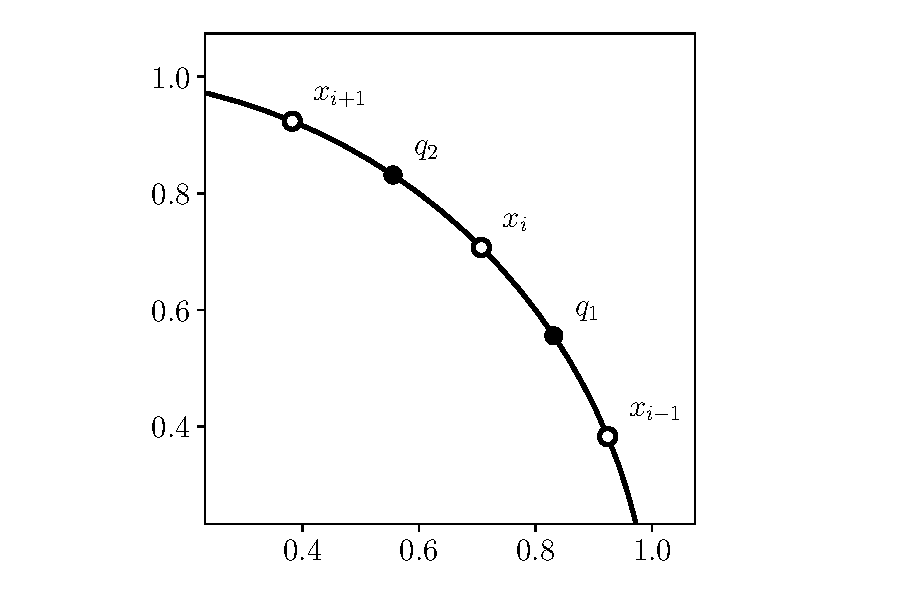
\includegraphics[width=0.8\textwidth]{figures/index.pdf}
    \caption{Bob places two points $q_1$ and $q_2$ in such a way
        on the unit circle, that they can be linearly seperated from the other
        points if and only if Alice didn't place a point at $x_i$.}
    \label{fig:index}
\end{figure}

In the proof of theorem~\ref{theorem:index}, we have already encountered
such a "degenerate" dataset, for which no sublinear sized coreset can be found,
consisting of only positive labels.
The next step of this work is to introduce a new complexity measure
for datasets in the context of probit regression, that allows us
to specify a broad class of datasets for which sublinear sized
coresets do exist and to show how such coresets can be constructed
for this class.
The idea behind this complexity measure goes back to
the work in~\cite{on-coresets}, where the authors introduced a similar
measure to describe a class of datasets that allow the construction
of sublinear coresets in the context of logistic regression.
We adapt this measure to the context of probit regression in the
following definition.

\begin{definition}($\mu$-complexity)
    \label{def:mu}
    Let $\mathcal{D}$ be a $d$-dimensional dataset of size
    $|\mathcal{D}|=n$ with scaled
    model matrix $Z \in \mathbb{R}^{n \times d}$, where
    $z_i \in \mathbb{R}^d$ constitutes the $i$-th
    row of $Z$ and let
    $w \in \mathbb{R}^n_{>0}$ be a vector of positive weights.
    Let $I_\beta^+ = \{i \in [n]:\ w_i z_i^T \beta > 0 \}$
    and let $I_\beta^- = \{i \in [n]:\ w_i z_i^T \beta < 0 \}$.
    Let
    \begin{equation*}
        \mu_w(\mathcal{D}) = \sup_{\beta \in \mathbb{R}^d \setminus \{0\}}
        \frac{\sum_{i \in I_\beta^+} w_i (z_i^T \beta)^2}
        {\sum_{i \in I_\beta^-} w_i (z_i^T \beta)^2}.
    \end{equation*}
    We call the dataset $\mathcal{D}$ with weight vector $w$
    $\mu$-complex, if there exists a $\mu \in \mathbb{R}$,
    such that $\mu_w(\mathcal{D}) \leq \mu$.
\end{definition}

There is a close relationship between $\mu$ and the linear
separability of a dataset as shown in the following theorem.

\begin{theorem}
    \label{theorem:mu-linear-separability}
    Let $\mathcal{D}$ be a $d$-dimensional dataset of size
    $|\mathcal{D}| = n$ like in definition~\ref{def:mu}
    and let $w \in \mathbb{R}^n_{>0}$ be a vector of
    positive weights.
    Then, the dataset
    $\mathcal{D}$ with weight vector $w$ is $\mu$-complex
    if and only if $\mathcal{D}$ is not linearly separable.
\end{theorem}
\begin{proof}
    We first prove the "$\Rightarrow$" direction, i.e. we show
    that if $\mathcal{D}$ is $\mu$-complex,
    then it is not linearly separable.
    We do this by proving the equivalent
    contraposition that if $\mathcal{D}$ is linearly separable,
    then it is not $\mu$-complex.

    Let $S_0 = \{i \in [n]:\ y_i = 0\}$ and $S_1 = \{i \in [n]:\ y_i = 1\}$
    like in definition~\ref{def:linear-separability}.
    If $\mathcal{D}$ is linearly separable, then there exists
    a $\beta \in \mathbb{R}^d \setminus \{0\}$, such that
    \begin{align*}
                    & \forall i \in S_0:\ x_i^T \beta \leq 0\quad \text{and}\quad \forall i \in S_1:\ x_i^T \beta \geq 0                       \\
        \iff        &                                                                                                                          \\
                    & \forall i \in S_0:\ (-1) x_i^T \beta \geq 0\quad \text{and}\quad \forall i \in S_1:\ x_i^T \beta \geq 0                  \\
        \iff        &                                                                                                                          \\
                    & \forall i \in S_0:\ (2y_i - 1) x_i^T \beta \geq 0\quad \text{and}\quad \forall i \in S_1:\ (2y_i - 1) x_i^T \beta \geq 0 \\
        \iff        &                                                                                                                          \\
                    & \forall i \in S_0:\ z_i^T \beta \geq 0\quad \text{and}\quad \forall i \in S_1:\ z_i^T \beta \geq 0                       \\
        \iff        &                                                                                                                          \\
                    & \forall i \in [n]:\ z_i^T\beta \geq 0                                                                                    \\
        \iff        &                                                                                                                          \\
                    & I_\beta^- = \{ i \in [n]:\ w_iz_i^T\beta < 0\} = \emptyset                                                               \\
        \iff        &                                                                                                                          \\
                    & \sum_{i \in I_\beta^-} w_i (z_i^T \beta)^2 = 0                                                                           \\
        \Rightarrow &                                                                                                                          \\
                    & \mu_w(\mathcal{D}) \geq \frac{\sum_{i \in I_\beta^+} w_i (z_i^T \beta)^2}
        {\sum_{i \in I_\beta^-} w_i (z_i^T \beta)^2} = \infty,
    \end{align*}
    which means that $\mathcal{D}$ is not $\mu$-complex.

    It now remains to prove the "$\Leftarrow$" direction, i.e. to
    show that if $\mathcal{D}$ is not linearly separable,
    then it is $\mu$-complex. Again, we do this by proving the
    equivalent contraposition that if $\mathcal{D}$ is not
    $\mu$-complex, then it is linearly separable.

    The first step in order to do so is to show that we can restrict the
    supremum in $\mu_w(\mathcal{D})$ to finite $\beta$ with
    $\lVert \beta \rVert = 1$:
    \begin{align*}
        \mu_w(\mathcal{D}) & = \sup_{\beta \in \mathbb{R}^d \setminus \{0\}}
        \frac{\sum_{i \in I_\beta^+} w_i (z_i^T \beta)^2}
        {\sum_{i \in I_\beta^-} w_i (z_i^T \beta)^2}                                         \\ & =
        \sup_{\beta \in \mathbb{R}^d \setminus \{0\}}
        \frac{\sum_{i \in I_\beta^+} \frac{1}{\lVert \beta \rVert^2}w_i (z_i^T \beta)^2}
        {\sum_{i \in I_\beta^-} \frac{1}{\lVert \beta \rVert^2} w_i (z_i^T \beta)^2}         \\
                           & =
        \sup_{\beta \in \mathbb{R}^d \setminus \{0\}}
        \frac{\sum_{i \in I_\beta^+} w_i \left(z_i^T \frac{\beta}{\lVert \beta \rVert}\right)^2}
        {\sum_{i \in I_\beta^-}  w_i \left(z_i^T \frac{\beta}{\lVert \beta \rVert}\right)^2} \\
                           & =
        \sup_{\tilde\beta \in \mathbb{R}^d,\ \lVert \tilde\beta \rVert = 1}
        \frac{\sum_{i \in I_\beta^+} w_i \left(z_i^T \tilde\beta \right)^2}
        {\sum_{i \in I_\beta^-}  w_i \left(z_i^T \tilde\beta \right)^2},
    \end{align*}
    which lets us conclude that even in the supremum, both expressions
    $\sum_{i \in I_\beta^+} w_i (z_i^T \beta )^2$
    and
    $\sum_{i \in I_\beta^-}  w_i (z_i^T \beta )^2$
    are finite.
    This means that if $\mathcal{D}$ is not $\mu$-complex, then
    the denominator must be zero, i.e. it must hold that there exists
    a $\beta \in \mathbb{R}^d \setminus \{0\}$ such that
    \begin{equation*}
        \sum_{i \in I_\beta^-}  w_i (z_i^T \beta )^2 = 0.
    \end{equation*}

    From here, we can follow the same chain of equivalences that we
    showed when proving the "$\Rightarrow$"-direction of the theorem,
    which leads us directly to the fact, that $\mathcal{D}$ in this case must
    be linearly separable, which concludes the proof.
\end{proof}

As we already noted in section~\ref{sec:parameter-estimation},
linear separability is also closely related to the existence
of the maximum likelihood estimate in the probit model.
The next theorem uses the relationship between $\mu$ and
linear separability to show the connection between $\mu$
and the existence and uniqueness of the maximum likelihood estimate.

\begin{theorem}
    Let $\mathcal{D}$ be a $d$-dimensional dataset of size
    $|\mathcal{D}| = n$ with model matrix $X \in \mathbb{R}^{n \times d}$
    and $rank(X) = d$, i.e. $X$ has full column rank.
    Then, the maximum likelihood estimate $\tilde\beta$ for the probit
    model exists and is unique if and only if $\mathcal{D}$ is $\mu$-complex.
\end{theorem}
\begin{proof}
    This is a direct corollary from theorem~\ref{theorem:probit-existence}
    and theorem~\ref{theorem:mu-linear-separability}.
    For model matrices with full column rank, the uniqueness of the
    MLE follows
    direclty from its existence, as shown in~\cite{wedderburn}.
\end{proof}

In the following parts of this work, we will derive efficient upper
bounds on the coreset size for $\mu$-complex datasets.
In order to do this, we first introduce a theoretic
framework that we use for the coreset construction which
is based on the concept of sensitivities.

\subsection{The Sensitivity Framework}

The sensitivity framework, which was first introduced
by~\cite{feldman-langberg-coresets} (see also
\cite{big-data-tiny-data} for a detailed overview),
is a method for constructing
provably small coresets by randomly sampling observations
from a dataset according to a probability distribution, that
emphasizes observations, which have a greater impact on the
objective function.

Instead of representing a dataset $\mathcal{D} = \{(x_i, y_i)\}_{i=1}^n$
as a set of labeled datapoints, the sensitivity framework
represents each point as a function that describes its
contribution to the objective function.
Recall, that in~\ref{sec:parameter-estimation}, we defined the
weighted objective function of the probit model as
$f_Z^w(\beta) = \sum_{i=1}^n w_i g(z_i^T \beta)$.
We will now associate each datapoint $(x_i, y_i)$ with the function
$g_i(\beta) := g(z_i^T \beta) = g((2y_i - 1)x_i^T \beta)$,
that describes its contribution to the total loss.
That way, we can equivalently represent a dataset in the context
of probit regression as a collection of loss functions
$F = \{g_1, ..., g_n\}$.

The idea behind the sensitivity framework is to draw a random
sample from this set of functions, where the sampling probability
of each function is proportional to its worst-case
contribution to the total loss for any $\beta \in \mathbb{R}^d$.
This worst-case importance is also called sensitivity and was first
introduced in~\cite{langberg-schulman-sensitivities}:

\begin{definition}[\cite{langberg-schulman-sensitivities}]
    \label{def:sensitivity}
    Let $F = \{ g_1, ..., g_n \}$ be a set of functions,
    $g_i: \mathbb{R}^d \rightarrow \mathbb{R}_{\geq 0}, \ i \in [n]$
    and let $w \in \mathbb{R}^n_{>0}$ be a vector of positive weights.
    The sensitivity of $g_i$ for $f_w(\beta) = \sum_{i=1}^n w_i g_i(\beta)$ is defined as
    \begin{equation*}
        \varsigma_i = \sup_{\beta \in \mathbb{R}^d, \ f_w(\beta) > 0} \frac{w_i g_i(\beta)}{f_w(\beta)}.
    \end{equation*}
    The total sensitivity, i.e. the sum of the sensitivities is $\mathfrak{S} = \sum_{i=1}^n \varsigma_i$.
\end{definition}

The true sensitivity $\varsigma_i$ of a function $g_i$ is usually unknown
and its computation can be expensive, because it involves solving the
original optimization problem, which was indicated in~\cite{braverman-feldman-coresets}.
For this reason, we are usually interested to find efficiently computable
upper bounds $s_i \geq \varsigma_i$ for the sensitivities and then
to draw samples proportional to the upper bounds $s_i$.
As we will see, as long as the sum $S = \sum_{i=1}^n s_i$ of the upper
bounds is sufficiently small, the coreset size will be small as well.

The second element of the sensitivity framework, which
\cite{feldman-langberg-coresets} related to the
concept of sensitivity sampling in order to obtain small coresets,
is the theory of range spaces and the VC-dimension.
Its relevant definitions are given below.

\begin{definition}[\cite{feldman-langberg-coresets}]
    A range space is a pair $\mathfrak{R} = (F, \textup{ranges})$, where F is a set
    and $\textup{ranges}$ is a family (set) of subsets of F.
\end{definition}

\begin{definition}[\cite{feldman-langberg-coresets}]
    The VC-dimension $\Delta(\mathfrak{R})$ of a range space
    $\mathfrak{R} = (F, \textup{ranges})$ is
    the size $|G|$ of the largest subset $G \subseteq F$ such that
    \begin{equation*}
        \left| \left\{ G \cap R \ | \ R \in \textup{ranges} \right\} \right|
        = 2^{|G|},
    \end{equation*}
    i.e. $G$ is shattered by $\textup{ranges}$.
\end{definition}

\begin{definition}[\cite{feldman-langberg-coresets}]
    Let $F$ be a finite set of functions mapping from $\mathbb{R}^d$ to $\mathbb{R}^{\geq 0}$.
    For every $\beta \in \mathbb{R}^d$ and $r \geq 0$, let
    \begin{equation*}
        \textup{range}(F, \beta, r) = \left\{ f \in F \ | \  f(\beta) \geq r  \right\}
    \end{equation*}
    and let
    \begin{equation*}
        \textup{ranges}(F) = \left\{ \textup{range}(F, \beta, r) \ | \ \beta \in \mathbb{R}^d, \ r \geq 0  \right\}.
    \end{equation*}
    Then we call $\mathfrak{R}_F := (F, \textup{ranges}(F))$ the range space induced by F.
\end{definition}

The following theorem is the basis of the sensitivity framework and
combines the theory of range spaces with the concept of
sensitivity sampling. Its original version goes back to
\cite{feldman-langberg-coresets}, but it was
further improved by
\cite{braverman-feldman-coresets}.
In this work, we will use the following variant by~\cite{big-data-tiny-data}:

\begin{theorem}[\cite{big-data-tiny-data}]
    \label{theorem:sensitivity-framework}
    Let $F = \{ g_1, ..., g_n \}$ be a set of functions,
    $g_i: \mathbb{R}^d \rightarrow \mathbb{R}_{\geq 0}, \ i \in [n]$
    and let $w \in \mathbb{R}^n_{>0}$ be a vector of positive weights.
    Let $\epsilon, \delta \in (0, \frac{1}{2})$.
    Let $s_i \geq \varsigma_i$ be upper bounds of the sensitivities and
    let $S = \sum_{i=1}^n s_i$.
    Given $s_i$, one can compute in time $O(|F|)$ a set
    $R \subseteq F$ of
    \begin{equation*}
        |R| \in O \left( \frac{S}{\epsilon^2} \left( \Delta \log S + \log \left( \frac{1}{\delta} \right) \right) \right)
    \end{equation*}
    weighted functions, such that with probability $1 - \delta$ we have
    for all $\beta \in \mathbb{R}^d$ simultaneously
    \begin{equation*}
        (1-\epsilon) \sum_{g_i \in F} w_i g_i(\beta) \leq \sum_{g_i \in R} u_i g_i(\beta) \leq (1 + \epsilon) \sum_{g_i \in F} w_i g_i(\beta).
    \end{equation*}
    Each element of $R$ is sampled independently with probability
    $p_j = \frac{s_j}{S}$ from $F$, $u_i = \frac{S w_j}{s_j |R|}$
    denotes the weight of a function $g_i \in R$ that corresponds to
    $g_j \in F$ and $\Delta$ is an upper bound on the
    VC-dimension of the range space $\mathfrak{R}_{F^\ast}$ induced by
    $F^\ast$, where $F^\ast$ is the set of functions $g_i \in F$
    scaled by $\frac{S w_i}{s_i |R|}$, i.e.
    $F^\ast = \left\{ \frac{S w_i}{s_i |R|} g_i(\beta) \ |\ i \in [n] \right\}$.
\end{theorem}

From this theorem, it follows that there are two things that have to be
done in order to find a small coreset for probit regression.

The first one is to find small and efficiently computable upper bounds
on the sensitivities and the second thing is to find a
small upper bound on the VC-dimension of the range space induced by $F^\ast$.
We will do both in the following section.

\subsection{Constructing the Coreset}

\subsubsection{Bounding the Sensitivity}

The first thing we need to do in order to find upper bounds on
the sensitivities is to find bounds on the function $g$,
which we do in the following two lemmas.

\begin{lemma}
    Let $g(x) = \ln \left( \frac{1}{1 - \Phi(x)}\right)$.
    Then, for all $x \geq 0$, it holds that:
    \begin{equation*}
        \frac{1}{2} x^2 \leq g(x).
    \end{equation*}
\end{lemma}
\begin{proof}
    We first show the claim for all $x \geq 1$, by using the following
    inequality:
    \begin{align*}
        \Phi(-x) & = \frac{1}{\sqrt{2 \pi}} \int_{-\infty}^{-x} \exp{ \left(-\frac{1}{2} z^2 \right)} dz       \\
                 & \leq \frac{1}{\sqrt{2 \pi}} \int_{-\infty}^{-x} -z \exp{ \left(-\frac{1}{2} z^2 \right)} dz \\
                 & = \frac{1}{\sqrt{2 \pi}} \exp{\left( -\frac{1}{2} x^2 \right)}                              \\
                 & \leq \exp{\left( -\frac{1}{2} x^2 \right)}.                                                 \\
    \end{align*}
    In the next step, we use this inequality to show that for $x \geq 1$:
    \begin{gather*}
        e^{g(x)} = e^{\ln \left( \frac{1}{1 - \Phi(x)} \right)} = \frac{1}{\Phi(-x)} \geq e^{\frac{1}{2} x^2}\\
        \iff \\
        g(x) \geq \frac{1}{2} x^2,
    \end{gather*}
    which proves the theorem for $x \geq 1$.

    Let us now turn to the case when $0 \leq x \leq 1$.
    Both $g(x)$ and $\frac{1}{2}x^2$ are monotonically increasing
    and continuous functions for $0 \leq x \leq 1$.
    Making use of the fact that $g(0) > \frac{1}{2}$, it follows
    for all $0 \leq x \leq 1$, that
    \begin{equation*}
        g(x) \geq g(0) > \frac{1}{2} = \max_{0 \leq x \leq 1} \frac{1}{2} x^2 \geq \frac{1}{2} x^2,
    \end{equation*}
    which concludes the proof.
\end{proof}

\begin{lemma}
    Let $g(x) = \ln \frac{1}{1 - \Phi(x)}$.
    Then, for all $x \geq 2$, it holds that:
    \begin{equation*}
        g(x) \leq x^2.
    \end{equation*}
\end{lemma}
\begin{proof}
    In~\cite{gaussian_bounds}, it was shown that the following inequality
    holds for all $x \geq 0$:
    \begin{equation*}
        \Phi(-x) \geq \frac{1}{\sqrt{2 \pi}} \frac{x}{x^2 + 1} e^{-\frac{1}{2} x^2}.
    \end{equation*}
    We can use this equality to establish that for all
    $x \geq 2$ it holds that:
    \begin{align*}
        e^{x^2} \cdot \Phi(-x) & \geq e^{x^2} \frac{1}{\sqrt{2 \pi}} \frac{x}{x^2 + 1} e^{-\frac{1}{2} x^2}                           \\
                               & = e^{\frac{1}{2} x^2} \frac{1}{\sqrt{2 \pi}} \frac{x}{x^2 + 1}                                       \\
                               & = e^{\frac{1}{2} x^2} \frac{1}{\frac{4}{3}\left( x^2 + 1 \right)} \frac{\frac{4}{3} x}{\sqrt{2 \pi}} \\
                               & \geq \frac{e^{\frac{1}{2} x^2}}{\frac{4}{3}\left( x^2 + 1 \right)}                                   \\
                               & \geq \frac{e^{\frac{1}{2} x^2}}{e^{\frac{1}{2} x^2}}                                                 \\
                               & = 1                                                                                                  \\
        \iff                                                                                                                          \\
        e^{x^2}                & \geq \frac{1}{1 - \Phi(x)}                                                                           \\
        \iff                                                                                                                          \\
        x^2                    & \geq \ln \left(\frac{1}{1 - \Phi(x)}\right) = g(x),
    \end{align*}
    which completes the proof.
\end{proof}

\begin{lemma}
    Let $\mathcal{D}$ be a $d$-dimensional and $\mu$-complex dataset of size
    $|\mathcal{D}|=n$ with scaled model matrix
    $Z \in \mathbb{R}^{n \times d}$ and let $w \in \mathbb{R}^d_{>0}$
    be a vector of positive weights.
    Let $F = \{g_1, ..., g_n\}$ be a set of functions with
    $g_i(\beta) = g(z_i^T \beta)$ and let
    $f_w(\beta) = \sum_{i=1}^n w_ig_i(\beta)$.
    Then, it holds that
    \begin{equation*}
        w_jg_j(\beta) \leq 2 \lVert U_j \rVert_2^2(1 + \mu)f_w(\beta) \quad
        \forall\ j \in \{i \in [n]:\ z_i^T \beta \geq 2 \},
    \end{equation*}
    where $U \in \mathbb{R}^{n \times d}$ is an orthonormal basis for
    the columnspace of $\sqrt{D_w}Z$ and $\sqrt{D_w} \in \mathbb{R}^{n \times n}$
    is a diagonal matrix, where the $i$-th diagonal element is equal to
    $\sqrt{w_i}$.
\end{lemma}
\begin{proof}
    Let $\sqrt{D_w} Z = UR$, where $U$ is an orthonormal basis for the columnspace
    of $\sqrt{D_w} Z$. Then, for all $j \in \{i \in [n]:\ z_i^T \beta \geq 2 \}$:
    \begin{align*}
        w_j g(z_j \beta)
         & = w_j g\left(\frac{\sqrt{w_j} z_j \beta}{\sqrt{w_j}}\right)
        = w_j g\left(\frac{U_j R \beta}{\sqrt{w_j}}\right)
        \leq w_j g\left(\frac{\lVert U_j \rVert_2 \lVert R \beta \rVert_2}{\sqrt{w_j}}\right)                   \\
         & = w_j g\left(\frac{\lVert U_j \rVert_2 \lVert U R \beta \rVert_2}{\sqrt{w_j}}\right)
        = w_j g\left(\frac{\lVert U_j \rVert_2 \lVert \sqrt{D_w} Z \beta \rVert_2}{\sqrt{w_j}}\right)           \\
         & \leq \lVert U_j \rVert_2^2 \lVert \sqrt{D_w} Z \beta \rVert_2^2
        \leq \lVert U_j \rVert_2^2 (1 + \mu) \lVert (\sqrt{D_w} Z \beta)^+ \rVert_2^2                           \\
         & = \lVert U_j \rVert_2^2 (1 + \mu) \sum_{i: \  \sqrt{w_i} z_i^T \beta > 0} w_i (z_i^T \beta)^2        \\
         & \leq 2 \lVert U_j \rVert_2^2 (1 + \mu) \sum_{i: \  \sqrt{w_i} z_i^T \beta \geq 0} w_i g(z_i^T \beta) \\
         & \leq 2 \lVert U_j \rVert_2^2 (1 + \mu) \sum_{i = 1}^n w_i g(z_i^T \beta)                             \\
         & = 2 \lVert U_j \rVert_2^2 (1 + \mu) f_w(\beta)
    \end{align*}
\end{proof}

\section{Data Streams}

Content.

\section{Experiments}

It is now time to investigate, how the two efficient algorithms that
we derived in the previous section behave on real world datasets,
both in the context of maximum likelihood estimation as well as
in a Bayesian setting.
In order to do so, we selected three benchmark datasets in advance
that will be used to compare both algorithms to each other as
well as to the baseline uniform sampling procedure, where each
sample is simply selected with equal probability.

It is important to emphasize, that the datasets used in the evaluation
are not a result of cherry picking: We selected the same datasets
as \cite{on-coresets} as well as \cite{coresets-strengthened}
in order to be comparable to other works in the field, without
testing in advance if our algorithms look good on them or not.

Finally, we note that all of the following experiments were
implemented in Python and executed on an
AMD Ryzen 7 2700x processor with 8 cores of 3.7GHz clock speed
and 16GB of RAM.
The code for all the experiments is open source and can be
found publicly accessible on Github.\footnote{
    \url{https://github.com/cxan96/efficient-probit-regression}
}

\subsection{Datasets}

The datasets that are used in the empirical evaluation of our
algorithms are called Covertype\footnote{
    \url{https://archive.ics.uci.edu/ml/datasets/Covertype}
}, Kddcup\footnote{
    \url{https://kdd.ics.uci.edu/databases/kddcup99/kddcup99.html}
} and Webspam\footnote{
    \url{https://www.csie.ntu.edu.tw/\~cjlin/libsvmtools/datasets/binary.html\#webspam}
} and are
all publicly available.

The Covertype dataset consists of $n=581012$ observations of 30x30m
forest patches of wilderness areas located in the
Roosevelt National Forest of Northern Colorado, USA.
The task is to predict the so called covertype of each of these
patches, i.e. the dominant tree species, based on $d=54$
observed features. There are seven distinct tree species that
appear in the dataset, so we have a multiclass problem. To transform
the problem into a binary classification problem that can be
subjected to a probit analysis, we adapted the task to distinguish the
tree species "Lodgepole Pine" from the other six species, thus
obtaining a balanced problem of $49\%$ positive vs $51\%$ negative
observations.
As an additional preprocessing step, all continuous features of the
dataset were scaled to have a mean of zero as well as unit variance.
In addition, an intercept column of all ones was appended to the data.

The Webspam datasets consists of $n=350000$ observations of
web pages, that can either be classified as spam or no spam, based
on the occurence of 254 distinct words on the web page.
$61\%$ of the observations in the dataset are labeled as spam
and the other $39\%$ are labeled as no spam. The task is to predict,
whether a given web page is spam or not.
The features consist of binary $0/1$ observations that indicate, if
a given word is present on a web page or not.
In a preprocessing step, words that are never present
in the dataset were removed, as well
as words that are only present on a single web page.
After preprocessing, the dataset that is subjected to the
experiments consists of $d=128$ binary features.
An intercept column of all ones was appended to the Webspam dataset
as well.

The Kddcup dataset consists of $n=494021$ observations of network
connections, where the task is to predict if a connection is
"good" or "bad", i.e. to distinguish, whether a hacker tried
to gain unauthorized
access to a network or whether someone tried to establish a
normal and authorized connection.
$80\%$ of the connections in the dataset are "bad" and the other
$20\%$ are "good" connections.
In a preprocessing step, $d=33$ continuous features
were retained from the data and scaled to a mean of zero and
unit variance. Just like the other datasets, an intercept column
of all ones was appended to the Kddcup data as well.

\subsubsection{A Visual Comparison of the Datasets}

Before we evaluate the three competing algorithms on each of
the datasets, we first make an attempt at uncovering some of
the structural characteristics of the data, that could
potentially help us to learn more about the situations in which
the algorithms perform well or might fail.

In order to do so, we first project each dataset onto
its first two principal components, which where obtained
as a result of a principal component analysis
\cite{principal-components}.
The first two principal components are orthogonal vectors that
represent the two directions of the data,
in which the highest variance occurs.
By projecting each datapoint onto the subspace spanned by
the first two principal components, we have
a way of visualizing the datasets in a two dimensional space, while
still retaining as much variance as possible, even though we are
reducing the dimensionality to only 2.

Next, we draw two distinct samples from the reduced datapoints,
each consisting of 500 points. The first one is a uniform sample,
where each datapoint is sampled with equal probability.
The second sample is drawn with probabilities that are proportional
to the statistical leverage scores of the observations with
respect to the original dataset, without applying a PCA.
Both of these samples are presented for each of the datasets in
figure~\ref{fig:dataset-comparison}.

\begin{figure}[ht!]
    \centering
    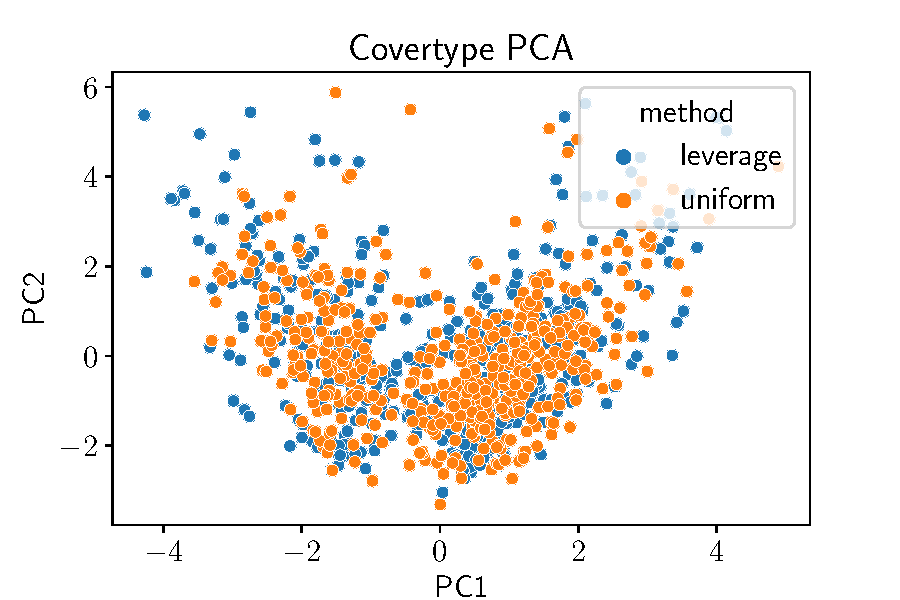
\includegraphics[width=.49\linewidth]{figures/covertype_pca.pdf}
    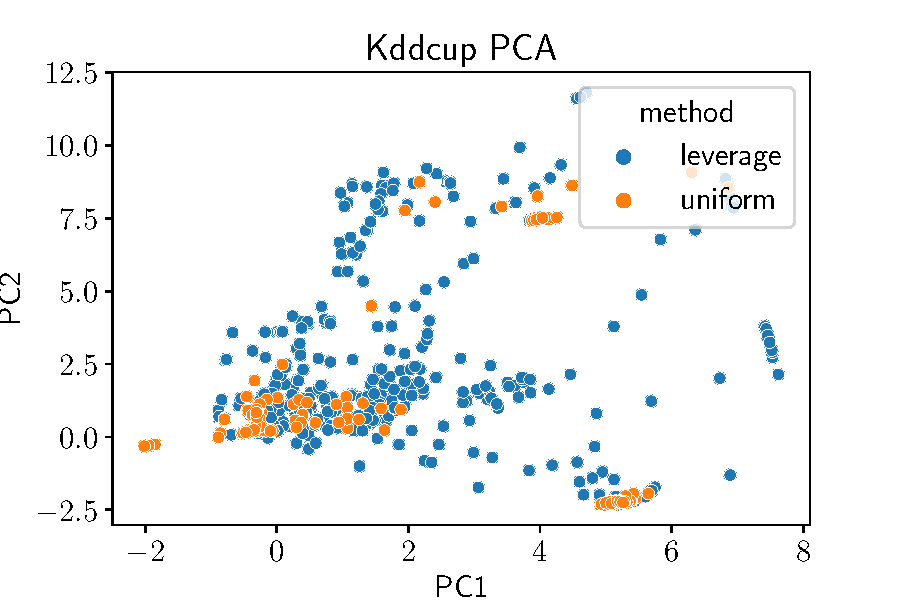
\includegraphics[width=.49\linewidth]{figures/kddcup_pca.pdf}
    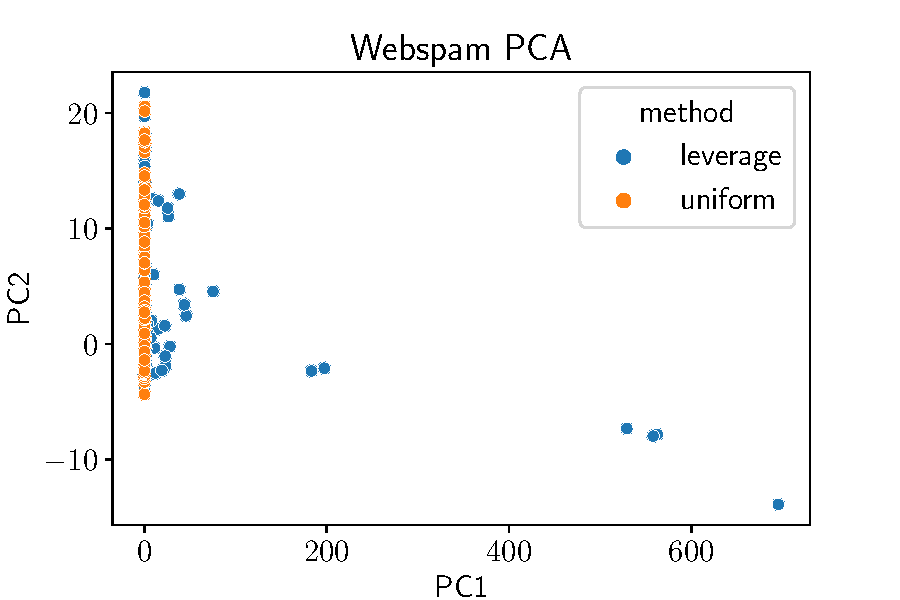
\includegraphics[width=.49\linewidth]{figures/webspam_pca.pdf}
    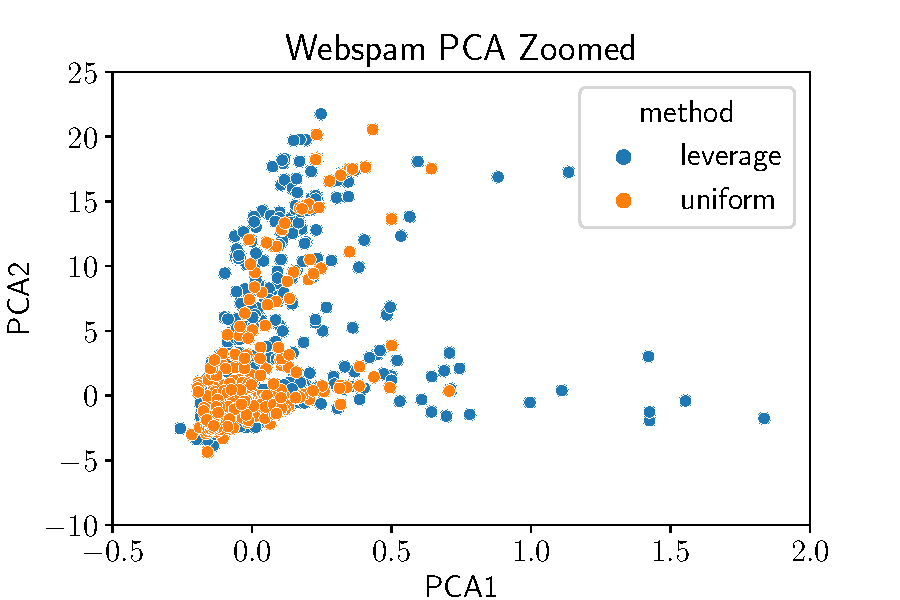
\includegraphics[width=.49\linewidth]{figures/webspam_pca_zoomed.pdf}
    \caption{The datasets are compared by projecting the datapoints
        onto the first two principal components and then drawing
        a random sample of 500 points (a) uniformly and (b) proportionally to the
        statistical leverage scores of the original data.}
    \label{fig:dataset-comparison}
\end{figure}

We can see, that the samples reveal some interesting characteristics
of the datasets. Starting with Covertype, we notice that there
hardly seems to be any difference between the uniform sample and
the leverage score sample. Taking into consideration, that the
statistical leverage scores assign a higher importance to
outliers or "unusual" datapoints, we can conclude that there don't
seem to be too many unusual observations within the Covertype
dataset, or else the two samples would differ more substantially.
It seems to be the case, that a uniform sample is already
sufficient to capture most of the inherent structure of the data,
without having to put extra weight on unusual datapoints, which
simply appear not to exist in this dataset.
Thus, from now on, it seems reasonable to think of the
Covertype dataset as being
a representative for such situations, where the data is
already quite uniformly distributed and not a lot of outliers are
present, i.e. where a uniform sample already seems to
yield good results.

In contrast to Covertype, the Kddcup dataset exhibits a different
picture. Here, we can see that the uniform sample and the leverage
score sample differ way more substantially than it was the case
for the Covertype dataset.
While the uniform sample only seems to occupy a very limited portion
of the feature space, most of it being a cluster of
many points close to the origin,
the leverage score sample covers a lot more
of the feature space,
indicating that there are a variety of unusual datapoints,
or outliers present,
which the uniform sample misses.
Thus, it seems that we can think of the Kddcup dataset as an
example of a situation,
where on the one hand, we have a lot of similar observations that
are concentrated within a comparatively small proportion of
the feature space, but on the other hand, we also have a
considerable amount of unique observations, which are scattered
around the feature space
while seemingly not belonging to any particular cluster.

Lastly, another interesting situation is presented to us when taking
a look at the two samples of the Webspam dataset.
What strikes the eye first, is that there seem to be some truly
extreme outliers present in the dataset, that the leverage score
sampling picked up on. Only by zooming in on the more crowded area
of the feature space and thereby ignoring those extreme outliers,
we can see the remaining parts of the two samples, which seem to
be rather similar, just like in the situation of the Covertype dataset.
It thus seems to be the case, that the Webspam dataset is an example
of a situation, where on the one hand, the vast majority of the
datapoints are concentrated around some region of the feature space,
but on the other hand, there are also a few hard hitting outliers present,
which exhibit enormous differences to the majority of the other
observations.

\subsection{Coreset-Based Maximum Likelihood Estimation}

We are now ready to investigate, how well our three algorithms
(two pass coreset construction, online coreset construction and
uniform sampling) perform at the task of data reduction
with the goal of estimating the
parameter vector of a probit model on the three datasets that
we just introduced via maximum likelihood estimation.
In order to do so, we present the following experimental setup:

For each of the datasets, we first obtain the objective function
$f(\beta)$ of the original optimization problem without applying
any data reduction and then solve the problem to find the
unique solution $\beta^{opt}$.
Next, we apply our data reduction algorithms in order to select
a small subset of the original data, yielding the reduced
objective function $\tilde{f}(\beta)$. We solve this
smaller optimization problem in order to obtain the solution
$\tilde{\beta}$. Our goal is to see, if the solution on the
reduced dataset, $\tilde{\beta}$, is also a good solution
for the original problem. In order to evaluate the approximation
quality, we compute what we call the approximation ratio:
\begin{equation*}
    \operatorname{approximation\ ratio} = \frac{f(\tilde{\beta})}{f(\beta^{opt})},
\end{equation*}
which always evaluates to a real number in the interval $[1, \infty)$.
The closer this value is to $1$, the better is the quality of
the approximation.

We run this procedure for each algorithm on each of the datasets
for multiple different reduction sizes. Because the algorithms
are not deterministic, we ran each of the experiments a total
of 51 times. The resulting medians as well as the normalized
inter quartile range can be seen in figure~\ref{fig:ratio-plots}.

\begin{figure}[ht!]
    \centering
    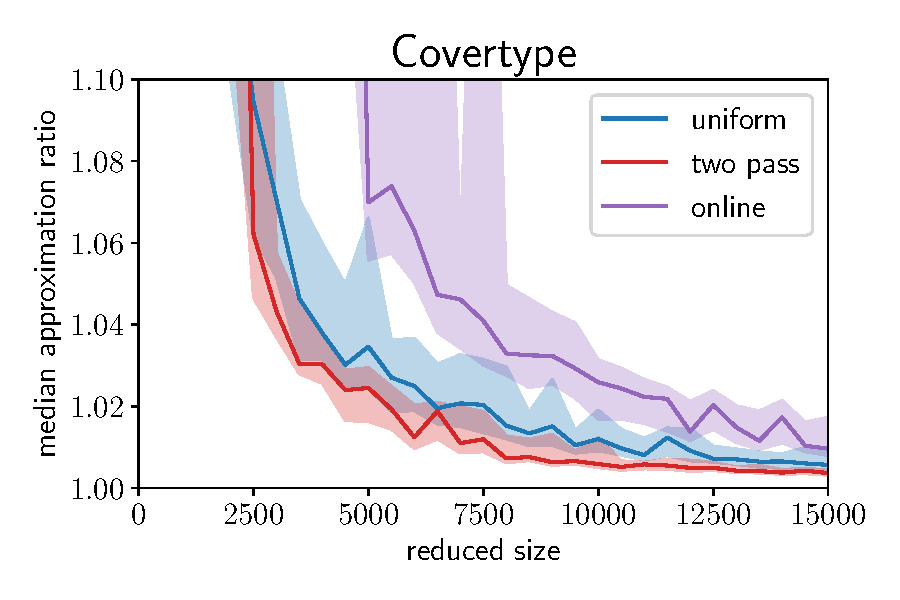
\includegraphics[width=.49\linewidth]{figures/covertype_ratio_plot.pdf}
    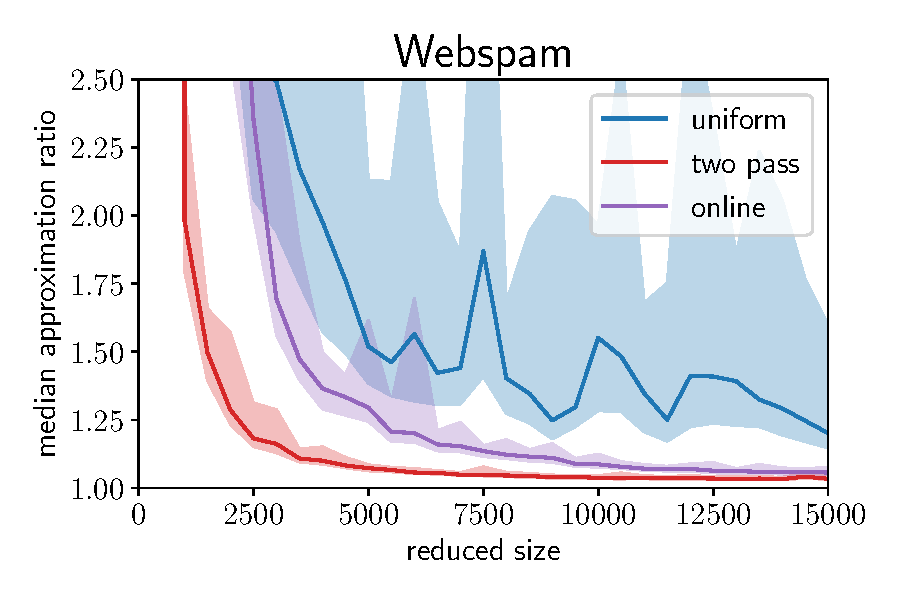
\includegraphics[width=.49\linewidth]{figures/webspam_ratio_plot.pdf}
    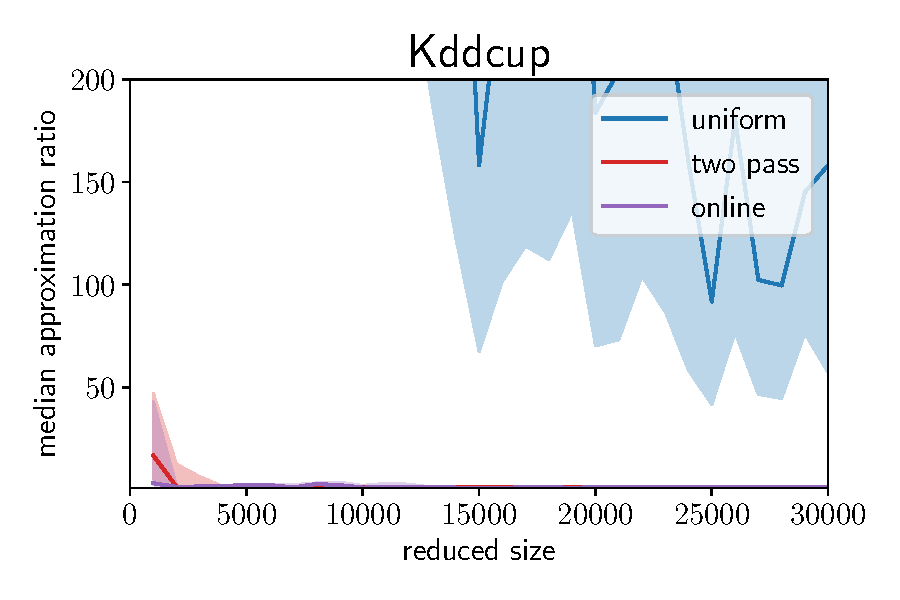
\includegraphics[width=.49\linewidth]{figures/kddcup_ratio_plot.pdf}
    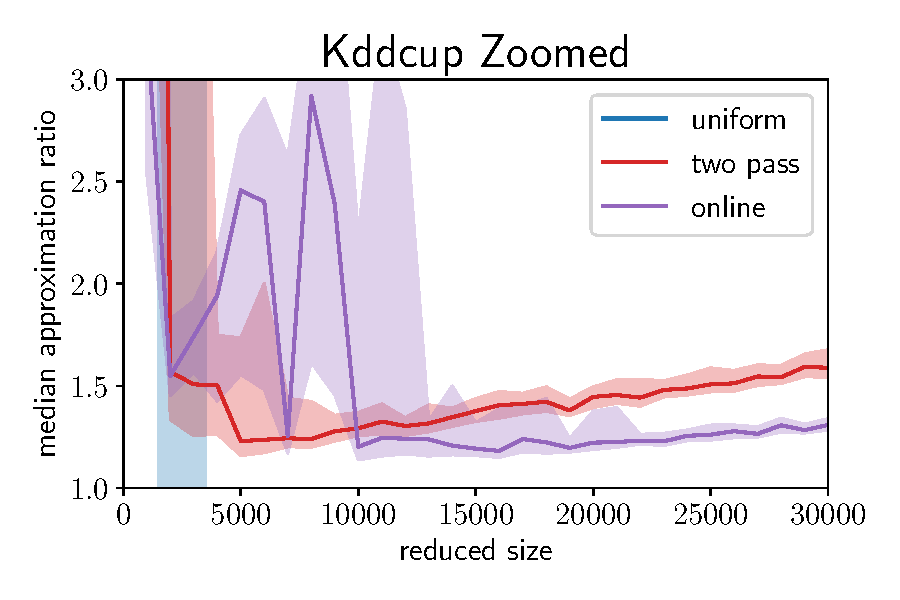
\includegraphics[width=.49\linewidth]{figures/kddcup_ratio_plot_zoomed.pdf}
    \caption{The medians as well as the normalized inter quartile
        ranges of the approximation ratios of the three
        algorithms uniform sampling, two pass coreset construction and
        online coreset construction on the datasets Covertype, Webspam
        and Kddcup for different data reduction sizes.
        For each reduction size, the experiments were repeated a
        total of 51 times.}
    \label{fig:ratio-plots}
\end{figure}

\subsubsection{Comparison of Approximation Quality}

Starting with the Covertype dataset, we can see that each algorithm
quickly reaches good approximation ratios of less than $1.02$
for subset sizes of only $15000$ datapoints, which are less than
$3\%$ of the original dataset.
Both, the uniform sampling as well as the two pass algorithm, are
close to each other in terms of approximation quality, although
the median ratio of the two pass algorithm is always better than
that of uniform sampling. The online algorithm performs worse than
the two competing algorithms, but it also quickly reaches a low
approximation ratio of less than $1.02$.
Interestingly, the fact that the results of our three algorithms
don't differ much on the Covertype dataset, could
be explained by our earlier
findings regarding the characteristics of the data.
For the Covertype dataset, we found that it could be a representative for
those situations, where the datapoints are already
quite homogeneously distributed, i.e. there
are not a lot of outliers, heavy hitters or other unusual points to worry
about and thus, a uniform sample can already be sufficient to
capture the relevant characteristics of the data.
Nevertheless, our two pass algorithm still outperformed the uniform
sampling procedure, albeit by only a small margin.

For the Webspam dataset, the picture looks a lot different. Here,
we can see for the first time that the uniform sampling algorithm
fails, while the two pass algorithm as well as the one pass
algorithms quickly reach low approximation ratios. On top of that,
the approximation ratios of the uniform sampling algorithm
exhibit a much higher degree of variation and thereby show a lot
less stability than the competing algorithms two pass and online.
Again, it is interesting to note, that these results could also
potentially be explained by our earlier observations:
When visualizing the Webspam dataset by using the first two
principal components, we already noticed that there are a few
extreme outliers present in the data. We also noticed, that
the uniform sample was unable to pick up on those outliers
and only concentrated on the bulk of the datapoints in
the center of the feature space. Now, in our
maximum likelihood experiments,
we can see that the uniform sampling procedure also
exhibits major weaknesses
for the Webspam dataset. It thus seems reasonable to assume,
that this is again happening because the uniform sampling
algorithm misses the extreme outliers, which could potentially have a
high impact on the objective function.
Both, the two pass algorithm as well as the online algorithm,
don't miss those important points thanks to their more
adaptive importance sampling distributions that also take
the statistical leverage scores into account, and therefore show a
stable convergence behavior towards low approximation rates.

The most dramatic differences between uniform sampling and the
competing algorithms can be observed when looking
at the results for the Kddcup dataset. Here, we can see that
uniform sampling fails terribly and doesn't even reach
approximation ratios lower than $50$. When zooming in, we can
see that our other two algorithms perform much better, although they
also seem to show some difficulties. It is especially interesting
to note, that the online algorithm seems to perform better than the
two pass algorithm, even though its approximations of the
statistical leverage scores are less accurate.
Together with our earlier observations of the structure of the
Kddcup dataset, it seems that Kddcup is a particularly difficult
dataset to compress. Even though the sampling methods that
also rely on the leverage scores clearly outperform the
uniform sampling algorithm, they also show difficulties with
regard to convergence. We should also note here, that the
maximum size of $30000$ points for the Kddcup dataset already
takes up more than $6\%$ of the whole dataset, which is more than
double as much as what was needed for the Covertype dataset to
achieve a much better approximation quality.
Thus, the Kddcup dataset seems to be more challenging for all the
competing algorithms, although the two pass algorithm and the
online algorithm handle the difficult conditions way better than
the uniform sampling algorithm.

\subsubsection{Comparison of Running Times}

We round off our first experiment with a discussion regarding the
runtimes of the algorithms compared to the time it takes to
solve the original problem without prior reduction, as well as
a discussion of the tradeoffs between approximation quality and
running time.

It must be noted, that the online coreset algorithm
had to be excluded from the comparison due to its
incomparably high running time of $O(nd^2)$, which would have
made it impossible to execute a sufficient number of experiments.
However, we remark that the advantage of the online algorithm isn't
necessarily its speed, but that it is able to construct coresets
even when two passes over the data are impossible and every sampling
decision has to be made immediately. Also, it might be possible
to drastically increase the efficiency of the online algorithm,
by running mutiple parallel instances of it on a distributed
cluster and then equally balancing the load of the incoming
data records between
each of the instances, but these possible adaptations are
left open for future work.

The total running times for obtaining the maximum
likelihood estimate of the probit model for each of the
datasets without applying any data reduction are given in
table~\ref{tab:running-times} and will serve as a
baseline for further discussions.

\begin{table*}[ht!]
    \centering
    \begin{tabular}{ l | l| l| l}
        \hline
                           & \textbf{Covertype} & \textbf{Kddcup} & \textbf{Webspam} \\ \hline
        Total running time & $535$ seconds      & $103$ seconds   & $447$ seconds    \\ \hline
    \end{tabular}
    \caption{The total running times that it takes to obtain the maximum
        likelihood estimator for each of the datasets.}
    \label{tab:running-times}
\end{table*}

In figure~\ref{fig:runtime-plots}, we present the
tradeoffs between approximation ratio and running time
for uniform sampling as well as for the fast two pass algorithm.
The reported times include the data reduction step as
well as the optimization step, in order to be able to
compare the times to the total running times without data reduction.

\begin{figure}[t]
    \centering
    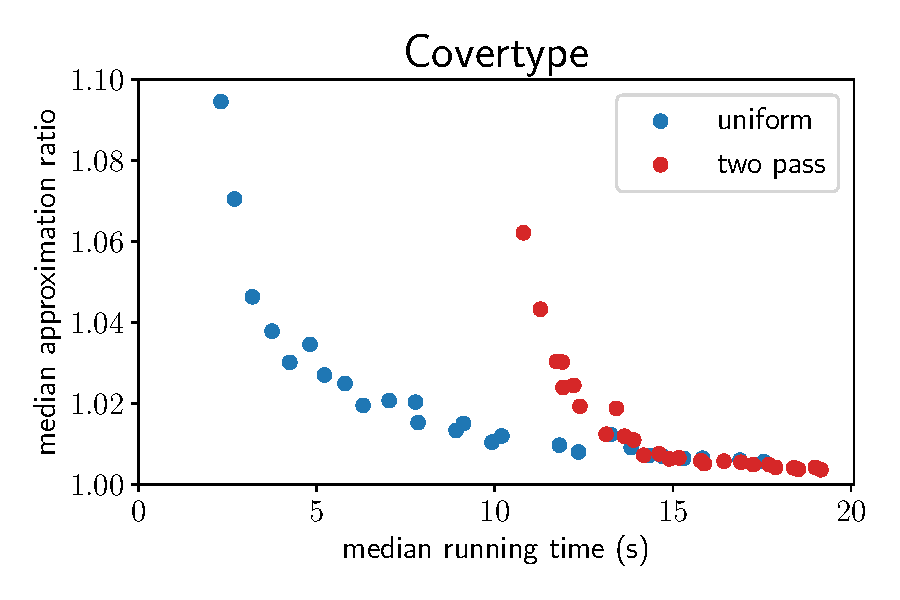
\includegraphics[width=.49\linewidth]{figures/covertype_runtime_plot.pdf}
    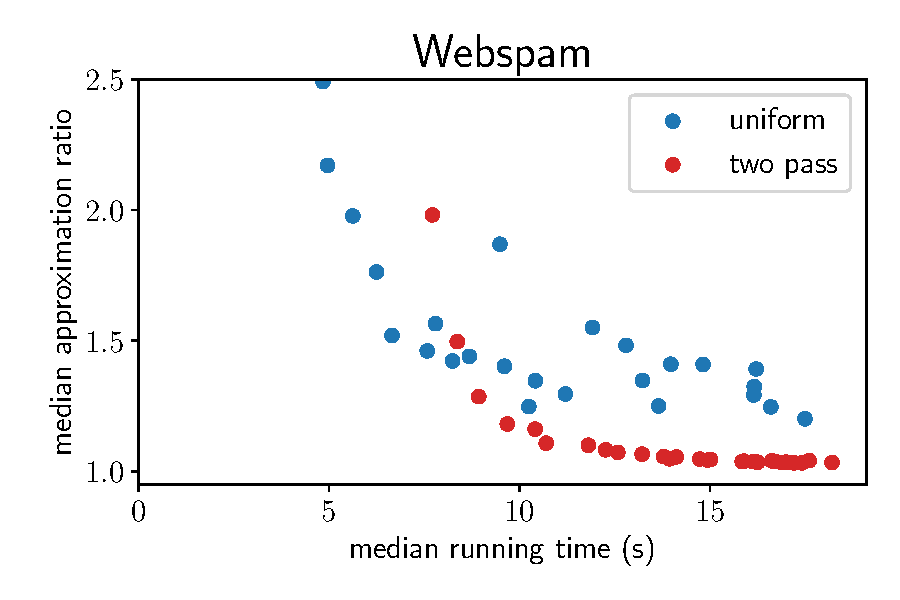
\includegraphics[width=.49\linewidth]{figures/webspam_runtime_plot.pdf}
    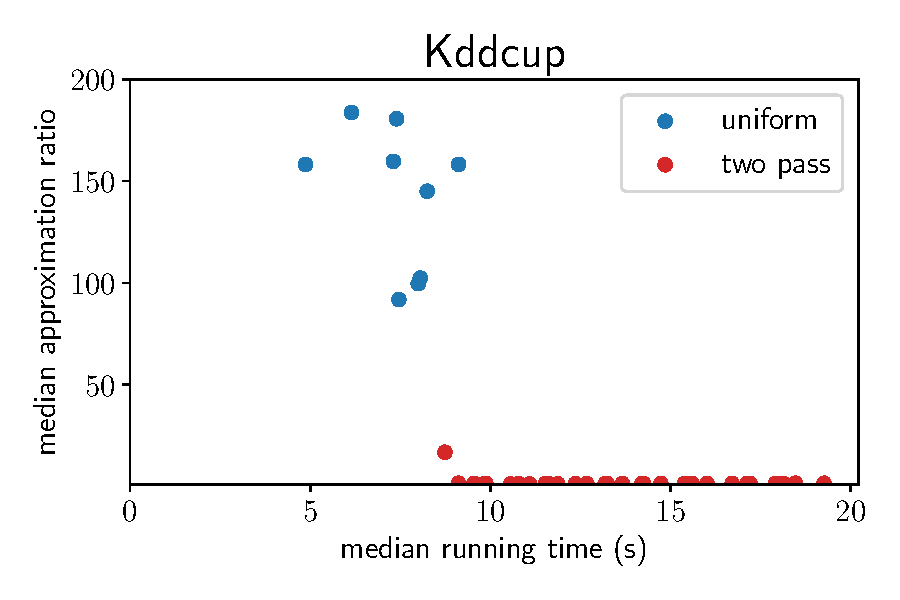
\includegraphics[width=.49\linewidth]{figures/kddcup_runtime_plot.pdf}
    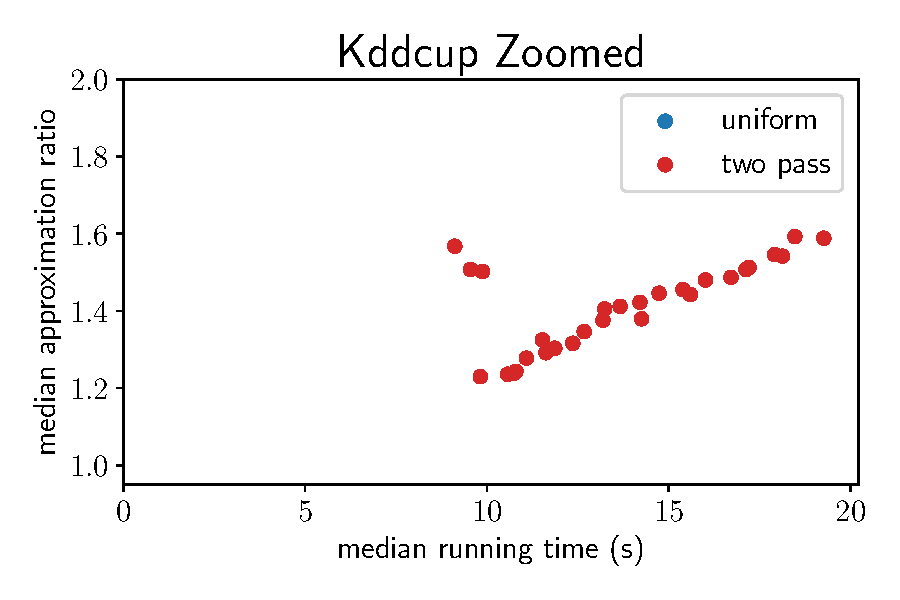
\includegraphics[width=.49\linewidth]{figures/kddcup_runtime_plot_zoomed.pdf}
    \caption{The plots show the tradeoffs between running time and
        approximation ratio for the uniform sampling algorithm and the
        fast two pass algorithm on our datasets.
        Every point represents the median in running time, as well
        as the median in approximation ratio, for a given
        data reduction size.
    }
    \label{fig:runtime-plots}
\end{figure}

When looking at the results for the Covertype dataset, we can see
that the uniform sampling algorithm outperforms the two pass
algorithm in terms of speed, but is unable to reach the same degree
of approximation quality as the two pass algorithm. The running times of
the uniform sampling procuedure range roughly between 1 and
10 seconds, but decent results are only achieved when investing
at least 5 seconds. On the other hand, the running times of the
two pass algorithm range between 10 and 20 seconds, thus taking
almost twice as long. But compared to the total running time
for the Covertype dataset without reduction, we can see that
even the two pass algorithm reduces the total running time
by more than $96\%$, from 535 seconds to less than 20 seconds.

Taking a look at the Webspam dataset, we can see an interesting
picture: Not only does the two pass algorithm show better
approximation rates than the uniform sampling algorithm, but
it also shows similar running times. Thus, for the Webspam dataset,
the two pass algorithm almost dominates the uniform sampling
in the two criterias, since it has similar running times but
achieves a better approximation quality.
For running times of 15 seconds, the fast two pass algorithm already
achieves decent results, thus we can say that the
original time for solving the unreduced problem was again reduced
by more than $96\%$, from 447 seconds to only 15 seconds.

In the case of Kddcup, the comparison is almost pointless, because
the uniform sampling fails. We only include these results to show
that the running times of the two pass algorithm consistently
range between 10 and 20 seconds, even when the data is
substantially less well behaved, as we showed for the
Kddcup dataset. Here, the time savings are not quite as impressive
as for the Covertype and the Webspam dataset:
The total running time was "only" reduced by more than $80\%$,
from 103 seconds to less than 20 seconds. Still, we can
consider this a decent win, especially when keeping
in mind that the uniform sampling algorithm failed completely.

To conclude the discussion of our first experiment, we can
say that the slightly increased running time of the two
pass algorithm compared to the uniform sampling algorithm
should be of no concern, because the few seconds in excess
runtime were always well compensated by substantial
gains in approximation quality. For each dataset,
the two pass algorithm is able to reduce the total
optimization time by more than $80\%$, even $96\%$ for
the Covertype and for the Webspam dataset.

\subsection{Coreset-Based Bayesian Inference}

The goal of our second experiment is to investigate, if our
algorithms can be successfully applied as a data reduction
step to cut down the computational cost of performing
a full Bayesian probit analysis on our three datasets.
In order to do so, we use the efficient Gibbs sampler
described earlier in section~\ref{sec:gibbs} to generate
samples with and without a preceding data reduction step using
our algorithms, and see how they compare to each other.
But before we can get into the full experimental setup,
we must note that in order to use the Gibbs sampler together
with our algorithms, it has to be slightly adapted
to account for the sample weights that are an
essential component of our coreset algorithms,
which is briefly covered in the next section.

\subsubsection{Adapting the Gibbs Sampler for Weighted Coresets}
\label{sec:gibbs-adaptation}

The first part of the Gibbs sampler that has to be slightly adapted
is the expression $B = (M^{-1} + X^TX)^{-1}$, where
$M \in \mathbb{R}^{d \times d}$
is the prior covariance matrix and
$X \in \mathbb{R}^{n \times d}$ is the model matrix.
When using our algorithms to draw a random sample of $k$
datapoints according to the distribution $p_1, ..., p_n$
and arranging them in a matrix $C \in \mathbb{R}^{k \times d}$,
the matrix $C$ is now random too, because it is the result of
drawing the random sample of our datapoints.
Our goal is now, to find weights $u_1, ..., u_n$ for our
data points, such that when $C$ is a random sample of the
reweighted datapoints $u_1x_1, ..., u_nx_n$, we have
\begin{equation*}
    E[C^TC] \overset{!}{=} X^TX,
\end{equation*}
where $X$ is the model matrix of our original unweighted datapoints.
We can accomplish this by calculating the expected value as follows:
\begin{align*}
    E[C^TC] & = E\left[\sum_{j=1}^k c_jc_j^T\right]
    = \sum_{j=1}^k \sum_{i=1}^n u_i^2 p_i x_i x_i^T \\
            & = k\sum_{i=1}^n u_i^2 p_i x_i x_i^T
    \overset{!}{=} \sum_{i=1}^n x_i x_i^T = X^TX.
\end{align*}
By comparing the coefficients, we see that
$u_i = \frac{1}{\sqrt{k p_i}}$ is the required weight.
Thus, when the Gibbs sampler is applied to a subset
$\mathcal{C}$ of our initial dataset, we need to multiply every
datapoint of the subset with the weight
$u_i = \frac{1}{\sqrt{k p_i}}$, before we can plug it into
the expression for obtaining $B$.

Next, we need to adapt the expression
$X^Ty^\ast$, where $y^\ast$ is the current vector of the latent
variables. We do this in a similar fashion, by asking
how we should reweight the original datapoints as well as the
latent variables in order to be unbiased, i.e. we want that
\begin{equation*}
    E\left[ C^T y_C^\ast \right] = X^T y^\ast,
\end{equation*}
where $y_C^\ast$ is the random sample of the latent variables that
is associated with the random sample in $C$.
Luckily, it turns out, that the weights that we obtained earlier
are also correct for adapting this expression:
\begin{align*}
    E\left[ C^T y_C^\ast \right] = E\left[ \sum_{j=1}^k c_j^T (y_C^\ast)_j \right]
    = \sum_{j=1}^k \sum_{i=1}^n u_i^2 p_i x_i^T y^\ast_i
    = k \sum_{i=1}^n \left(\frac{1}{\sqrt{kp_i}}\right)^2 p_i x_i^T y^\ast_i
    = X^T y^\ast.
\end{align*}

It follows, that when using the Gibbs sampler in conjunction
with our algorithms, we have to reweight our sample with weights
$u_i = \frac{1}{\sqrt{k p_i}}$ both when obtaining $X^TX$ as
well as $X^Ty^\ast$.

\subsubsection{Experimental Setup}

We used a similar experimental setup
as in \cite{scalable-bayesian-logreg} and
\cite{bayesian-regression}:
First, we arbitrarily selected a relatively uninformative
prior distribution of
\begin{equation*}
    \beta \sim \mathcal{N}(0, 10 \cdot \mathcal{I}),
\end{equation*}
where $\mathcal{I}$ is the identity matrix.
Next, we used the Gibbs sampler
to generate a sample of the full posterior
distribution without applying any data reduction for each
of the three datasets.
Each of the three full posterior samples has a size of $10000$,
and for each of the datasets, a different
burn in value was selected. For Covertype, a burn in
of 200 was sufficient, 2000 was needed for Kddcup and 3000
for Webspam.

Next, we applied our algorithms to each of the datasets
for a variety of reduction sizes and ran the adapted version of
the Gibbs sampler (see Section~\ref{sec:gibbs-adaptation} above)
on the reduced data, obtaining a posterior sample of size 1000
for each data reduction size. The burn in values for
the reduced samples were set to be
the same as for the original unreduced data.

Our goal is now to compare the posterior samples that were
obtained by running the Gibbs sampler on the reduced data
to the posterior samples that were obtained from the
original data.
In order to do so, we use a total of three different measures.

The first measure of approximation quality that we
apply compares the mean
of the original posterior distribution without data reduction to
the mean of the posterior distribution with a prior data reduction step,
by evaluating the expression
$\lVert \mu_\beta - \widetilde{\mu}_\beta \rVert_2$,
where $\mu_\beta$ is the mean of the original posterior and
$\widetilde{\mu}_\beta$ is the mean of the reduced posterior.

Likewise, our second measure compares the covariance matrices of
the two samples by evaluating the expression
$\lVert \Sigma_\beta - \widetilde{\Sigma}_\beta \rVert_2$,
where $\Sigma_\beta$ is the covariance matrix of the original
posterior sample without data reduction and
$\widetilde{\Sigma}_\beta$ is the covariance matrix of the
posterior sample with data reduction. The norm $\lVert \cdot \rVert_2$
refers to the $\ell_2$ matrix norm, which is equal to the
largest singular value.

Our third measure is the maximum mean discrepancy (MMD,
see for example \cite{mmd}),
which was also applied in \cite{scalable-bayesian-logreg}.
The MMD was originally intended to be a test statistic for the
problem of testing, if two samples come frome the same
distribution or not.
In order to do so, the idea behind the MMD is to transform
both samples into a higher dimensional space and then to
compare the means of the samples in the new space.
The MMD is then the resulting difference of the means in the
higher dimensional space. It follows, that the higher the
MMD, the more different the two samples are.
In order to transform the samples
into the higher space, the authors of
\cite{scalable-bayesian-logreg} used a so called polynomial
kernel function, and to stay comparable to them, we
use a polynomial kernel as well.

\subsubsection{Comparison of Approximation Quality}

Figure~\ref{fig:bayes-plots-norm-cov} shows the results of our
experiment for the measures
$\lVert \mu_\beta - \widetilde{\mu}_\beta \rVert_2$, which
we from now on call mean distance and
$\lVert \Sigma_\beta - \widetilde{\Sigma}_\beta \rVert_2$,
which we from now on call cov distance.
The results for the MMD can be found in Figure~\ref{fig:bayes-plots-mmd}.

\begin{figure}[ht!]
    \centering
    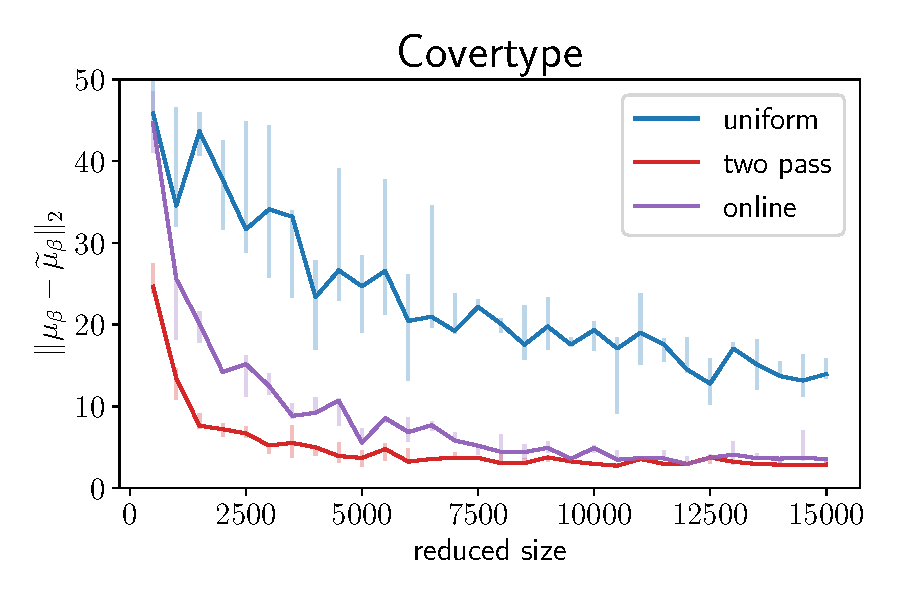
\includegraphics[width=.49\linewidth]{figures/covertype_bayes_plot_norm.pdf}
    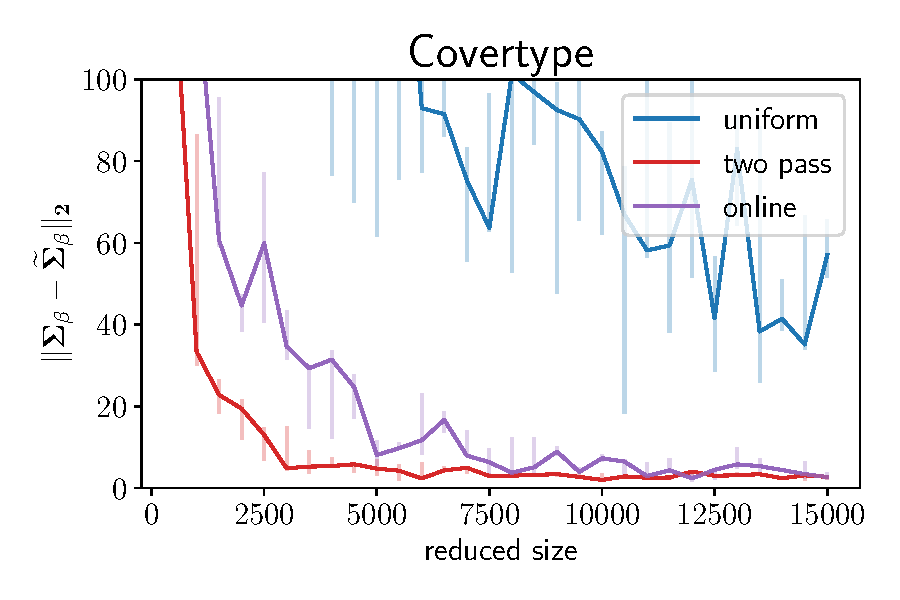
\includegraphics[width=.49\linewidth]{figures/covertype_bayes_plot_matrix_norm.pdf}
    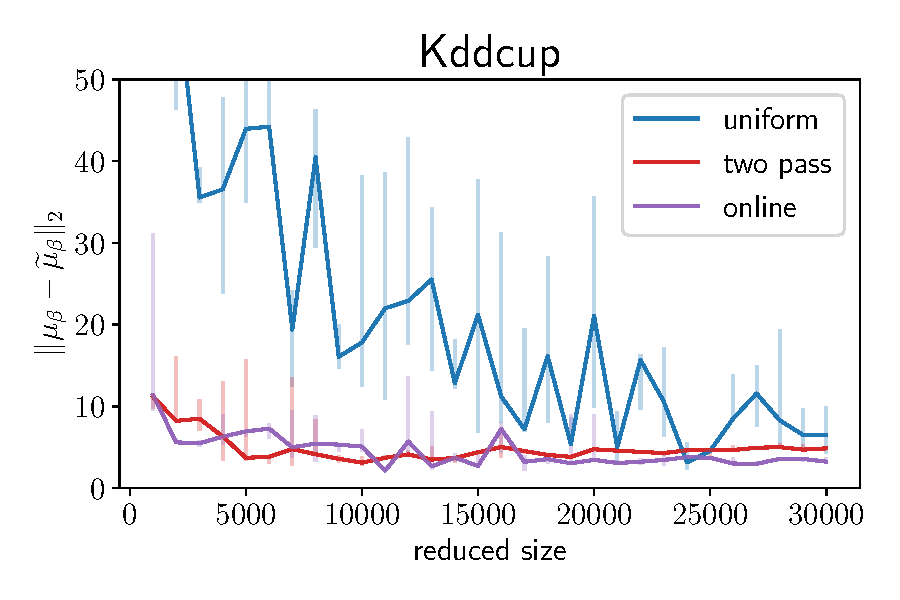
\includegraphics[width=.49\linewidth]{figures/kddcup_bayes_plot_norm.pdf}
    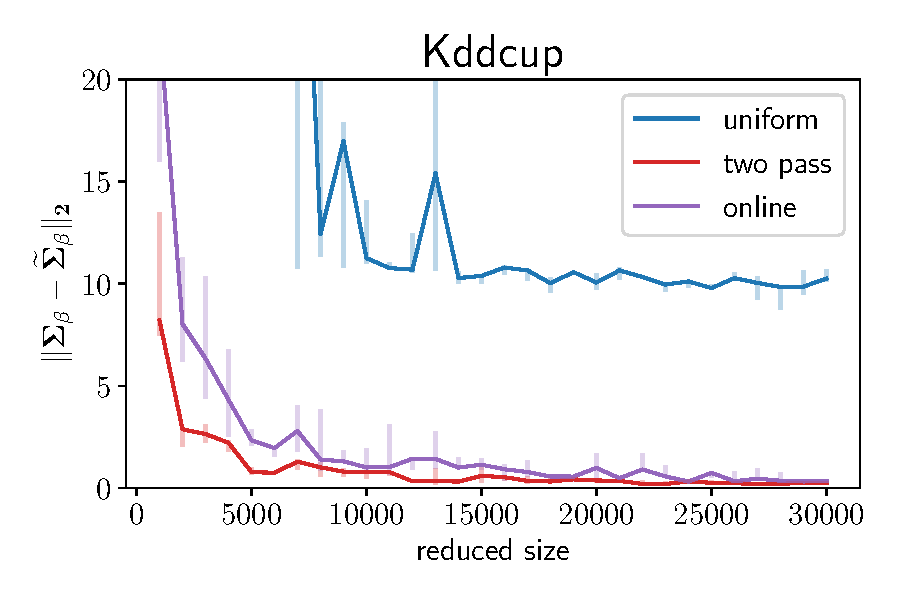
\includegraphics[width=.49\linewidth]{figures/kddcup_bayes_plot_matrix_norm.pdf}
    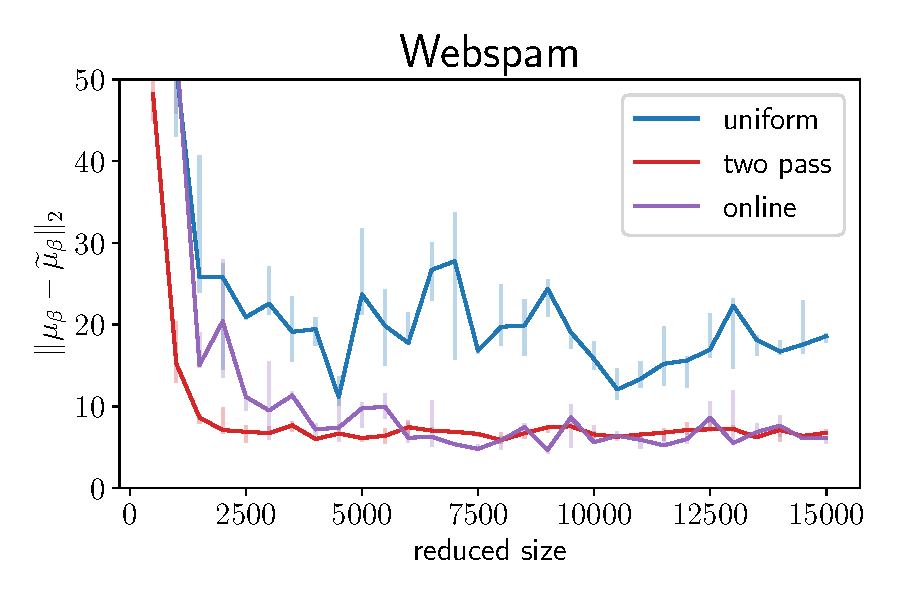
\includegraphics[width=.49\linewidth]{figures/webspam_bayes_plot_norm.pdf}
    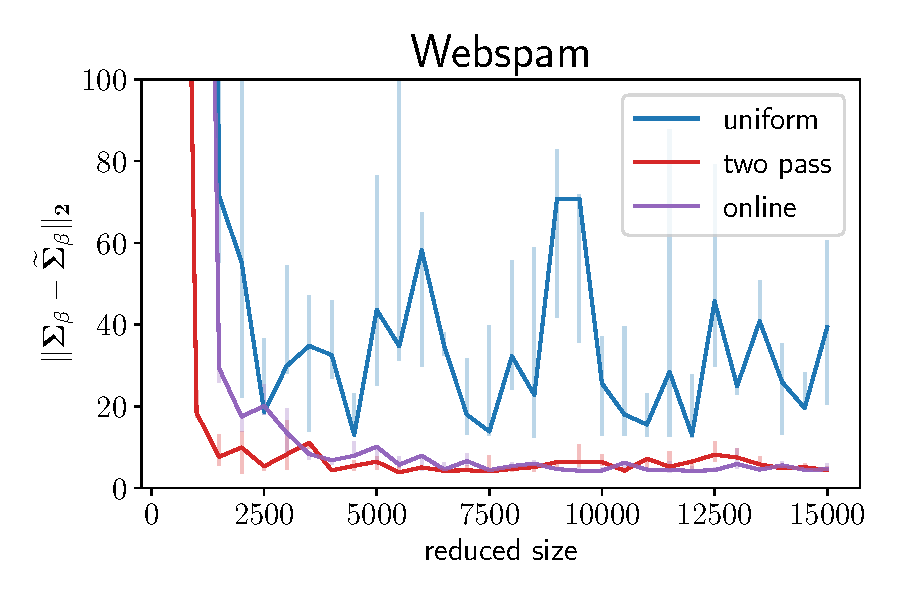
\includegraphics[width=.49\linewidth]{figures/webspam_bayes_plot_matrix_norm.pdf}
    \caption{In the left column, we see the mean distance between the posterior
        distribution sampled after running our algorithms and
        the original posterior distribution sampled without data
        reduction. In the right column, we see the cov distance for
        our algorithms. Every experiment was repeated a total
        of 5 times, and the solid lines represent the
        medians. The lower and upper error bars indicate the
        $25\%$ quantile as well as the $75\%$ quantile, respectively.}
    \label{fig:bayes-plots-norm-cov}
\end{figure}

\begin{figure}[ht!]
    \centering
    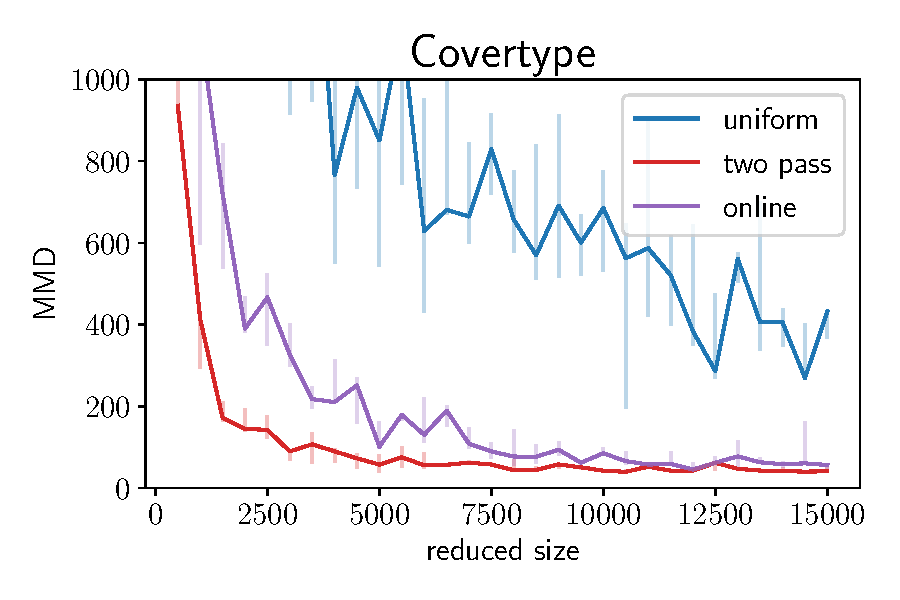
\includegraphics[width=.49\linewidth]{figures/covertype_bayes_plot_mmd.pdf}
    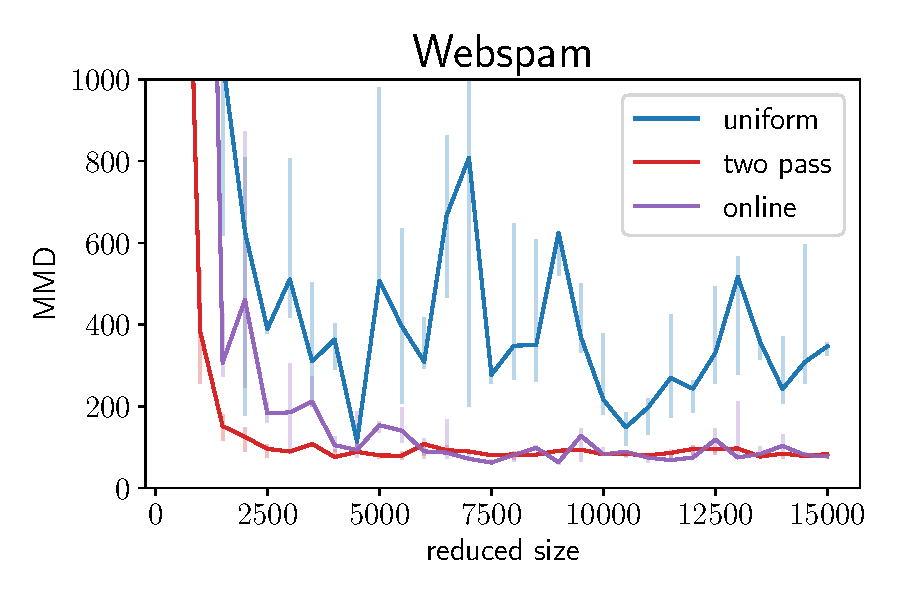
\includegraphics[width=.49\linewidth]{figures/webspam_bayes_plot_mmd.pdf}
    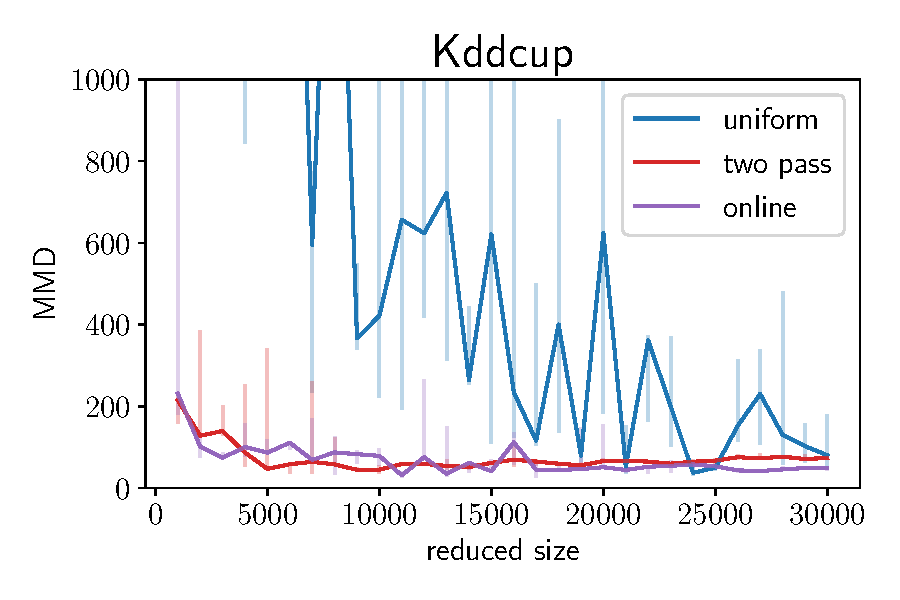
\includegraphics[width=.49\linewidth]{figures/kddcup_bayes_plot_mmd.pdf}
    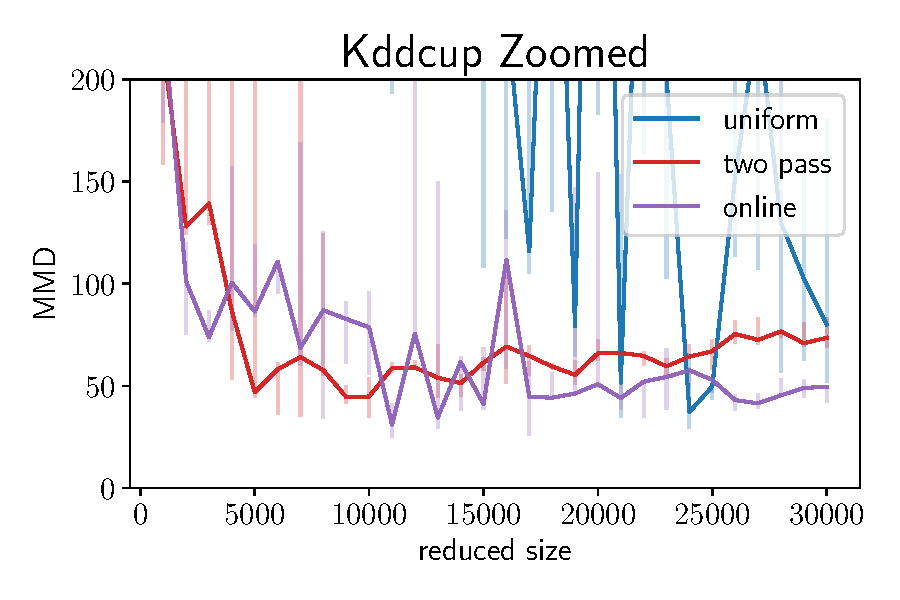
\includegraphics[width=.49\linewidth]{figures/kddcup_bayes_plot_mmd_zoomed.pdf}
    \caption{The MMD for each dataset and multiple data reduction
        sizes. Every experiment was repeated a total
        of 5 times, and the solid lines represent the
        medians. The lower and upper error bars indicate the
        $25\%$ quantile as well as the $75\%$ quantile, respectively.}
    \label{fig:bayes-plots-mmd}
\end{figure}

We can see, that for every dataset, the uniform sampling procedure
seems to show substantial weaknesses in approximation quality of
the posterior distribution compared to our two leverage score
based algorithms.
Even for the Covertype dataset, which we characterized to be
relatively well behaved for uniform sampling, our algorithms
perform considerably better for each of the three measures.

\begin{figure}[ht!]
    \centering
    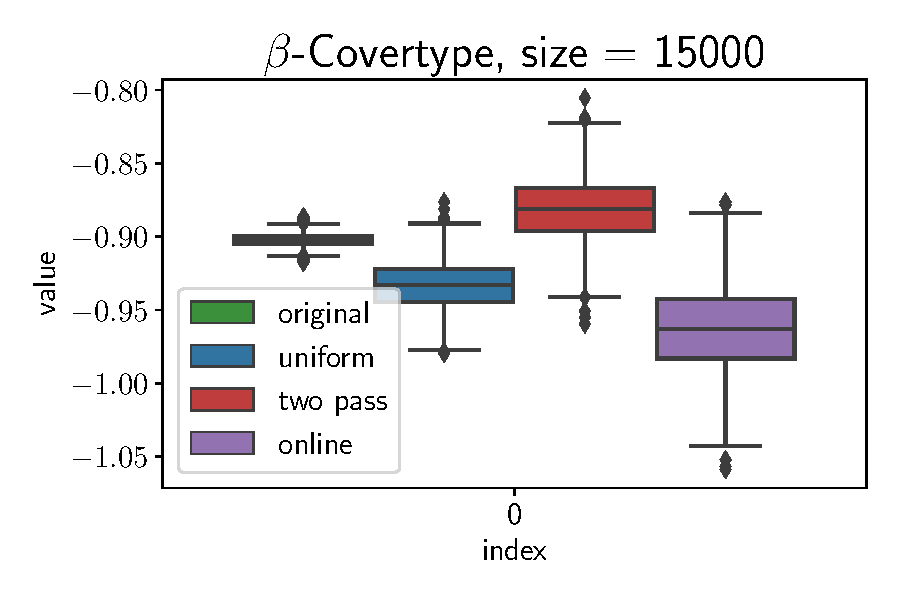
\includegraphics[width=.49\linewidth]{figures/covertype_coefficients/covertype_coefficients_0.pdf}
    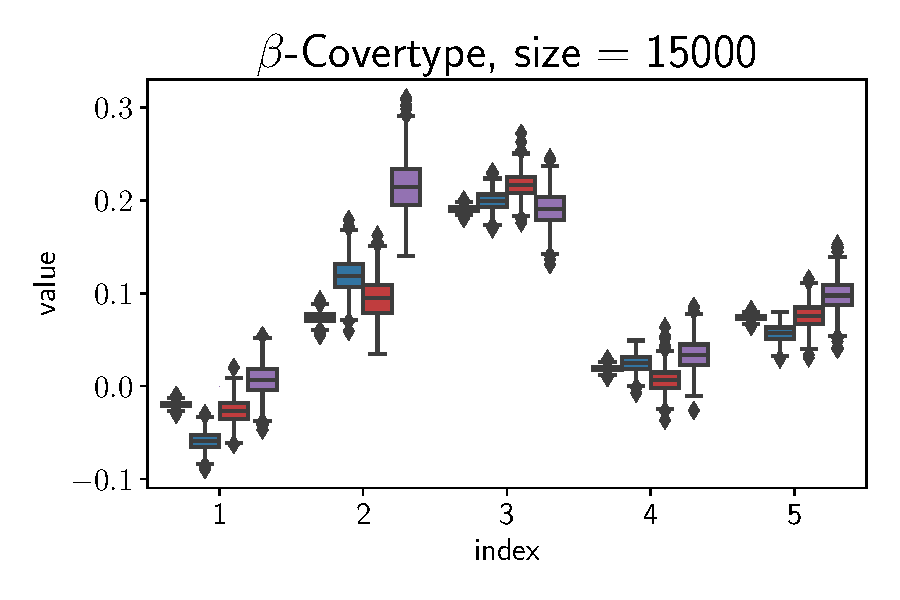
\includegraphics[width=.49\linewidth]{figures/covertype_coefficients/covertype_coefficients_1.pdf}
    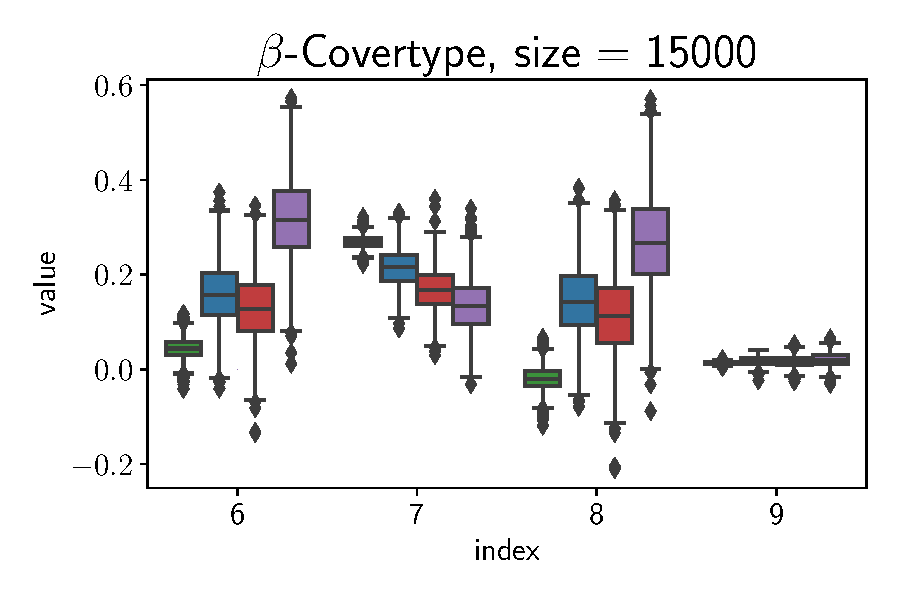
\includegraphics[width=.49\linewidth]{figures/covertype_coefficients/covertype_coefficients_6.pdf}
    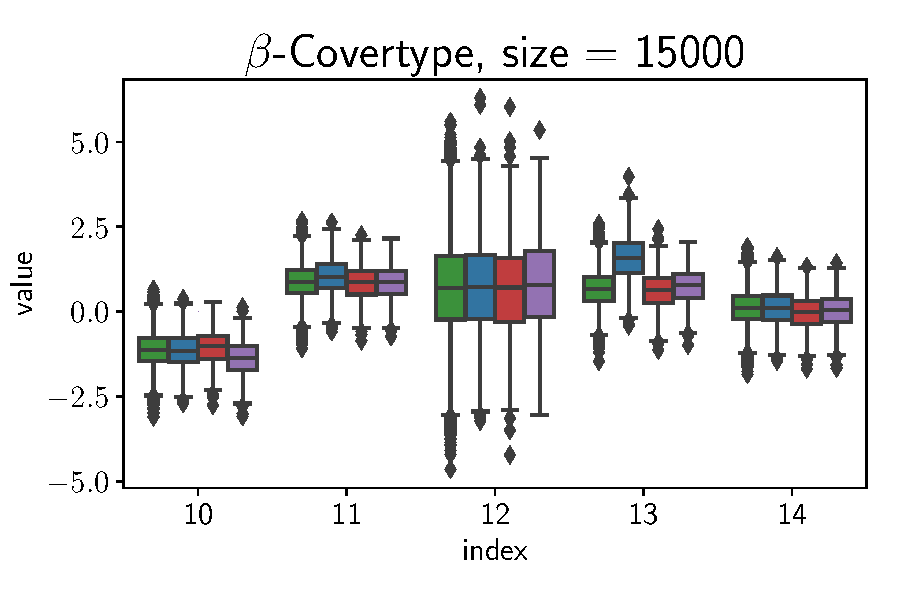
\includegraphics[width=.49\linewidth]{figures/covertype_coefficients/covertype_coefficients_10.pdf}
    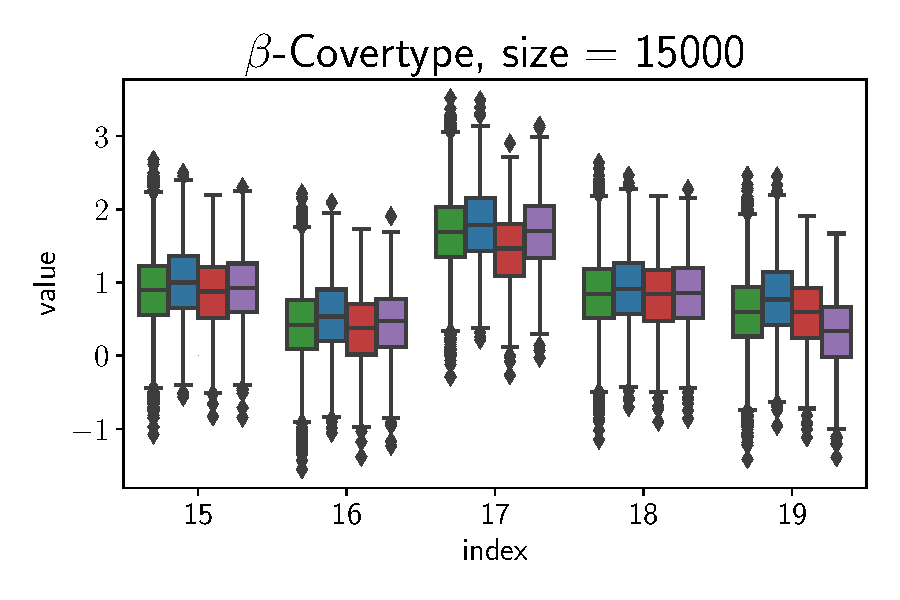
\includegraphics[width=.49\linewidth]{figures/covertype_coefficients/covertype_coefficients_15.pdf}
    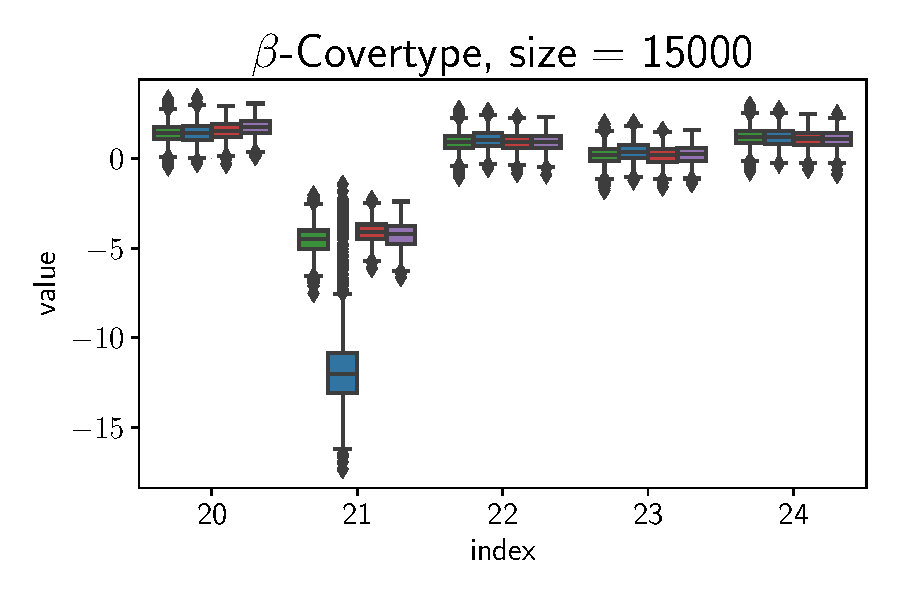
\includegraphics[width=.49\linewidth]{figures/covertype_coefficients/covertype_coefficients_20.pdf}
    \caption{}
    \label{fig:covertype-coefficients-1}
\end{figure}

\begin{figure}[ht!]
    \centering
    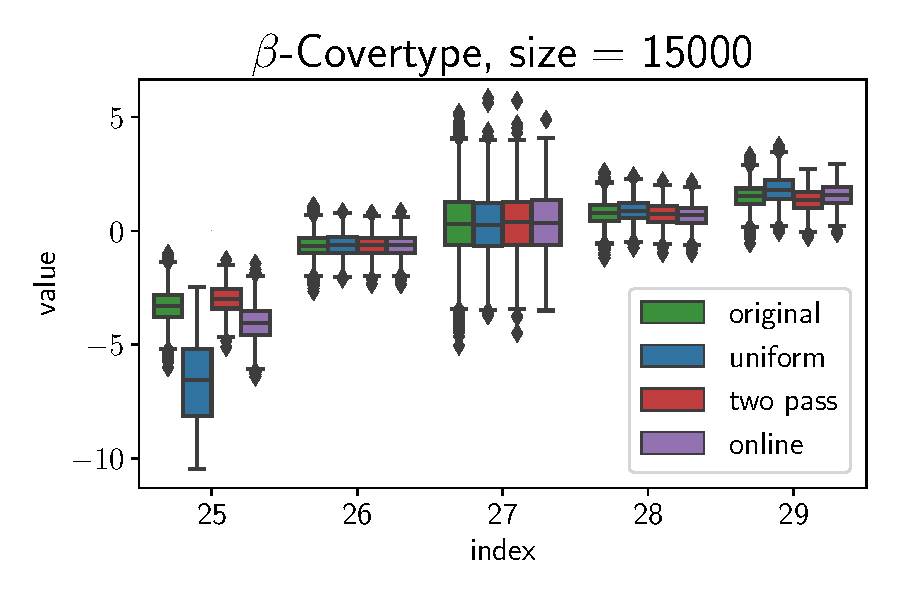
\includegraphics[width=.49\linewidth]{figures/covertype_coefficients/covertype_coefficients_25.pdf}
    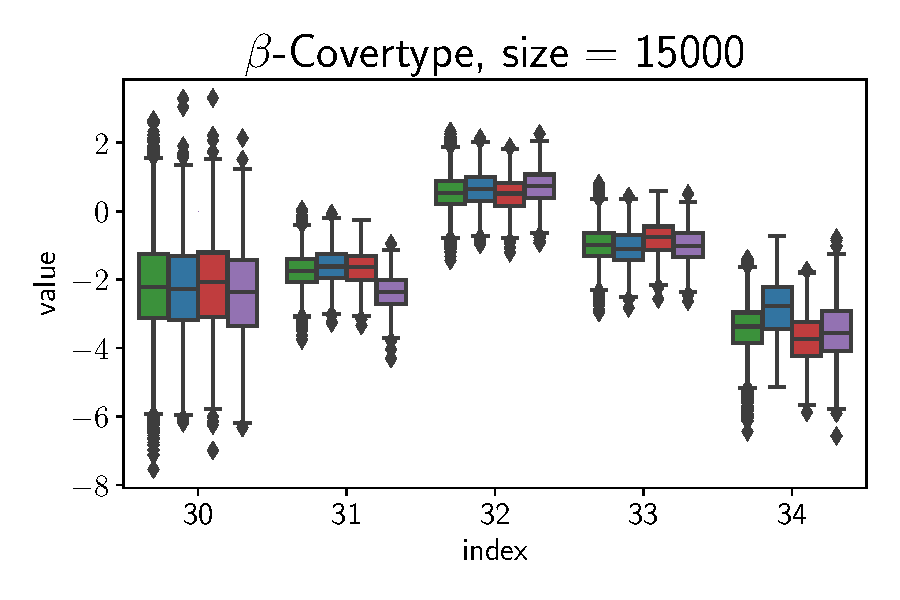
\includegraphics[width=.49\linewidth]{figures/covertype_coefficients/covertype_coefficients_30.pdf}
    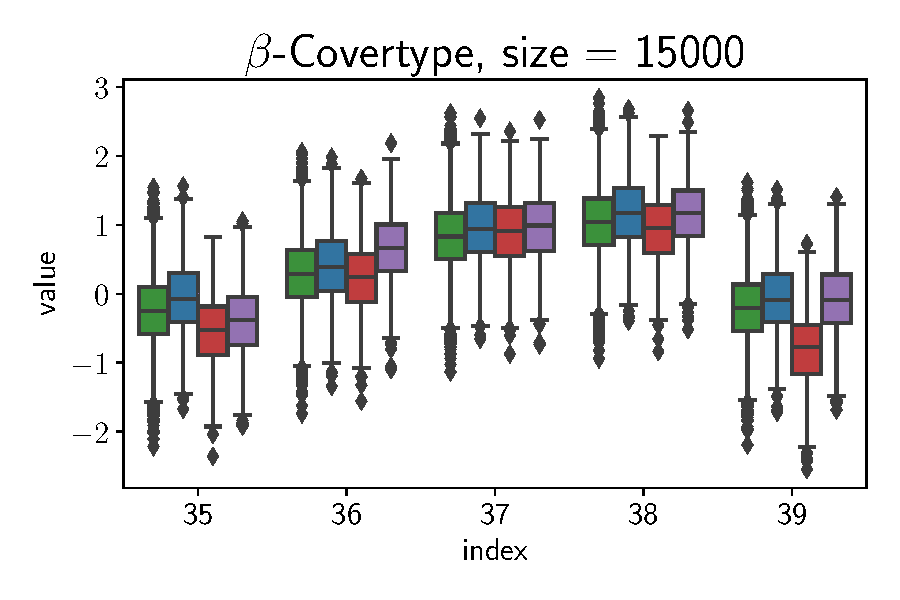
\includegraphics[width=.49\linewidth]{figures/covertype_coefficients/covertype_coefficients_35.pdf}
    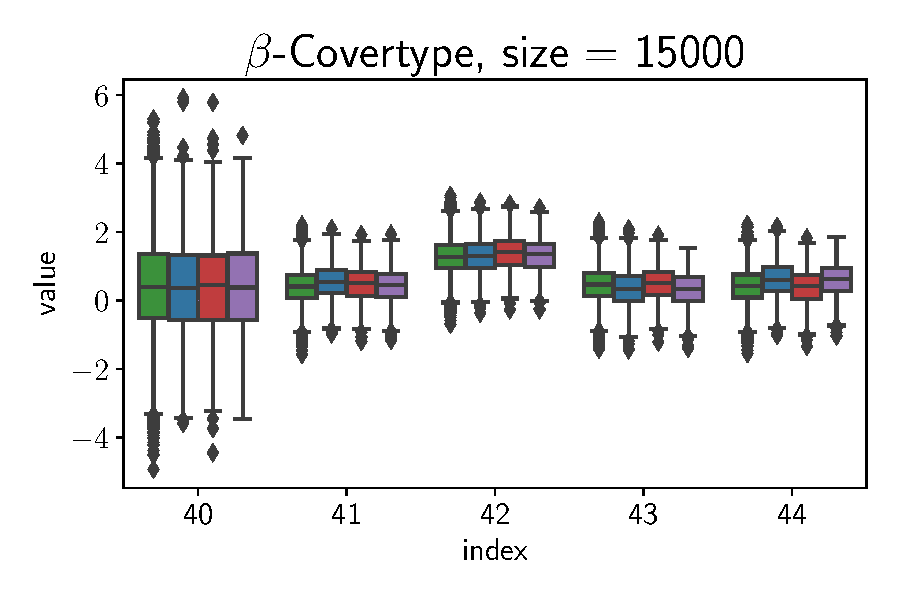
\includegraphics[width=.49\linewidth]{figures/covertype_coefficients/covertype_coefficients_40.pdf}
    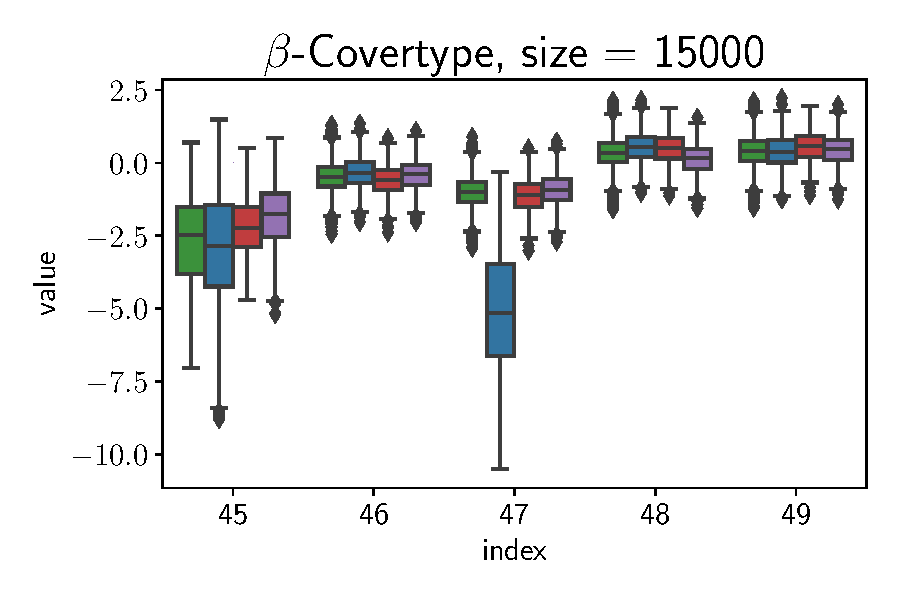
\includegraphics[width=.49\linewidth]{figures/covertype_coefficients/covertype_coefficients_45.pdf}
    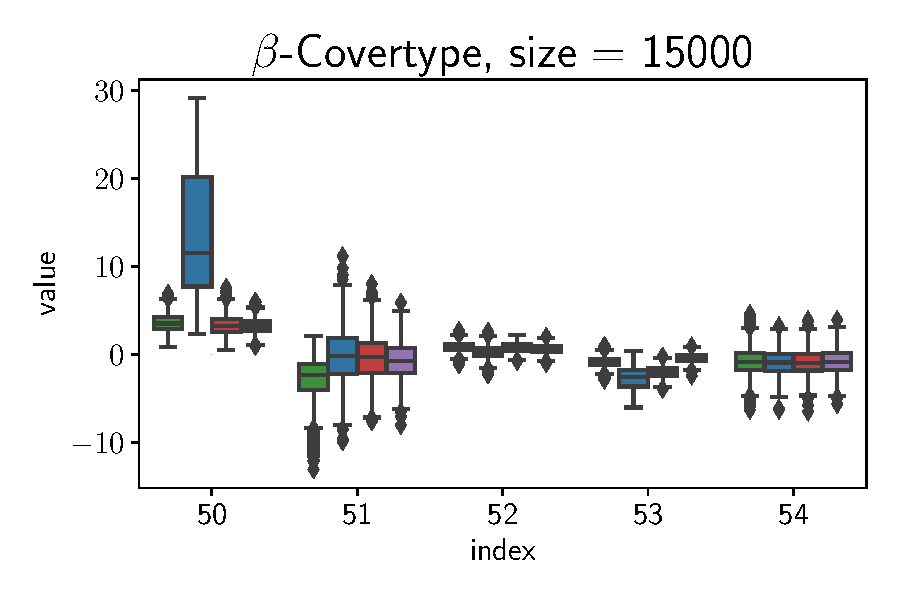
\includegraphics[width=.49\linewidth]{figures/covertype_coefficients/covertype_coefficients_50.pdf}
    \caption{}
    \label{fig:covertype-coefficients-2}
\end{figure}

\subsubsection{Comparison of Running Times}

\begin{table*}[ht!]
    \centering
    \begin{tabular}{ l | l| l| l}
        \hline
        \textbf{Method} & \textbf{Size} & \textbf{Dataset} & \textbf{samples per second} \\ \hline
        No reduction    & 581012        & Covertype        & 1.5                         \\ \hline
        two pass        & 15000         & Covertype        & 36                          \\ \hline
        uniform         & 15000         & Covertype        & 46                          \\ \hline
        two pass        & 1000          & Covertype        & 116                         \\ \hline
        uniform         & 1000          & Covertype        & 176                         \\ \hline
        No reduction    & 494021        & KDDCup           & 4                           \\ \hline
        two pass        & 15000         & KDDCup           & 21                          \\ \hline
        uniform         & 15000         & KDDCup           & 107                         \\ \hline
        two pass        & 1000          & KDDCup           & 85                          \\ \hline
        uniform         & 1000          & KDDCup           & 619                         \\ \hline
        No reduction    & 350000        & Webspam          & 2                           \\ \hline
        two pass        & 15000         & Webspam          & 13                          \\ \hline
        uniform         & 15000         & Webspam          & 28                          \\ \hline
        two pass        & 1000          & Webspam          & 60                          \\ \hline
        uniform         & 1000          & Webspam          & 84                          \\ \hline
    \end{tabular}
    \caption{TODO}
    \label{tab:running-times-bayes}
\end{table*}


\section{Contributions}

We conclude this work by recapitulating the contributions we delivered
during our analysis of coreset-based data reduction algorithms
for the probit model.

As a first step, we were able to show, that not all dataset allow
for obtaining small $(1 \pm \epsilon)$ approximations of the
probit loss function, but we
managed to overcome this obstacle by restricting our analysis to only
those datasets, where a probit model can successfully be applied
by using the method of maximum likelihood estimation.
Further, we extended the notion of $\mu$-complexity by
\cite{on-coresets} to the realm of probit analysis and showed, how
$\mu$-complexity is linked to the existence and uniqueness of the
maximum likelihood estimator of the probit model, making it a
necessary precondition for our subsequent advances in constructing the
data reduction algorithms.

In the next step, we introduced the notion of coresets as well as
the sensitivity framework and thereby outlined a roadmap, which we
would follow towards our ambition of finding our first coreset
construction algorithm.
Adhering to the theory of the sensitivity framework, we first
showed that sampling proportionally to the statistical leverage
scores yields small sensitivity bounds and we also managed to
control the VC dimension of our problem
by applying the technique of leverage
score rounding, thus arriving at our first provably correct
coreset algorithm that can reduce a $\mu$-complex dataset to
a size with a leading term in only $O(\mu d^2 \log(n))$.

Having successfully constructed our first data reduction algorithm,
we quickly noticed that there were some substantial issues regarding
its running time and efficiency,
that still needed improvement. In order to do so, we applied the sketching
methods outlined in \cite{leverage-scores-drineas} and
\cite{woodruff-2017} to obtain our fast two pass coreset algorithm.
In an attempt to adapt the fast two pass algorithm to situations,
where two passes are impossible and each sampling decision has to
be made immediately, we made use of the ideas in
\cite{online-row-sampling} and \cite{tensor-factorization}
to obtain an online coreset algorithm, which only requires a single
pass over the dataset.

To round off our work and demonstrate the practical applicability
of our algorithms, we conducted a variety of experiments
on three real world datasets, both in the domain of maximum
likelihood estimation as well as in the Bayesian setting.
Our experiments showed, that the algorithms we derived
outperform the baseline uniform sampling algorithm with
regards to approximation quality in
nearly all situations by a significant margin.
Only in terms of running time, the uniform sampling algorithm
still reigns superior, although its gains in execution speed
are overshadowed by its glaring instabilities and oftentimes
mediocre results in approximation quality.
Thus, for the data analysis practitioner who seeks reliable
methods for reducing vast amounts of data with the goal
of efficiently carrying out a probit analysis,
our algorithms were demonstrated to be
viable options, both in the frequentist domain of maximum
likelihood estimation and in the Bayesian setting as well.


\paragraph{Situation:}
We have $n$ data points $(x_i, y_i), \ i=1,...,n$ with
$x_i \in \mathbb{R}^d$ and $y \in \{ -1, 1\}$.

\paragraph{Probit Model:}
$y_i$ is a realization of the random variable $Y_i$.
$Y_1, ..., Y_n$ are independent.
The distribution of $Y_i$ is as follows:
\begin{align*}
    P(Y_i = 1 | x_i; \beta)  & = \Phi(x_i^T \beta)                          \\
    P(Y_i = -1 | x_i; \beta) & = 1 - \Phi(x_i^T \beta) = \Phi(-x_i^T \beta)
\end{align*}
where $\beta \in \mathbb{R}^d$.
It follows that
\begin{align*}
    P(Y_i = y_i | x_i; \beta) = \Phi(y_i x_i^T \beta)
\end{align*}

\paragraph{Likelihood:}
The likelihood of a parameter vector $\beta$ is given as follows:
\begin{equation*}
    L(\beta) = \prod_{i=1}^n P(Y_i = y_i | x_i; \beta) = \prod_{i=1}^n \Phi(y_i x_i^T \beta)
\end{equation*}
The negative log-likelihood that we wish to minimize is:
\begin{equation*}
    \mathcal{L}(\beta) = -\sum_{i=1}^n \log \Phi(y_i x_i^T \beta)
\end{equation*}

\paragraph{The weighted case:}
We introduce sample weights $w_i \in \mathbb{R}_{>0}$
comprising a weight vector $w \in \mathbb{R}_{>0}^n$.
Further, let $g(z) = -\log \Phi(-z)$.
The objective function now becomes:
\begin{equation*}
    f_w(\beta) = \sum_{i=1}^n w_i g(-y_i x_i^T \beta)
\end{equation*}
To make the notation easier, we define $z_i = -y_i x_i^T$ and introduce
the matrix $Z \in \mathbb{R}^{n \times d}$ with row vectors $Z_i = z_i$.
This gives us:
\begin{equation*}
    f_w(\beta) = \sum_{i=1}^n w_i g(z_i \beta)
\end{equation*}

\begin{lemma}
    Let $g(z) = -\log \Phi(-z)$. Then it holds for all $z \geq 0$ that:
    $$
        \frac{1}{2} z^2 \leq g(z)
    $$
\end{lemma}
\begin{proof}
    The following relationship holds for all $z \geq 1$:
    \begin{align*} 
        \Phi(-z) & = \frac{1}{\sqrt{2 \pi}} \int_{-\infty}^{-z} \exp{ \left(-\frac{1}{2} x^2 \right)} dx                 \\
                 & \leq \frac{1}{\sqrt{2 \pi}} \int_{-\infty}^{-z} \frac{-x}{z} \exp{ \left(-\frac{1}{2} x^2 \right)} dx \\
                 & = \frac{1}{\sqrt{2 \pi} z} \exp{\left( -\frac{1}{2} z^2 \right)}                                      \\
                 & \leq \exp{\left( -\frac{1}{2} z^2 \right)}                                                            \\
    \end{align*}
    We therefore have for $z \geq 1$:
    $$
        e^{g(z)} = e^{-\log \Phi(-z)} = \frac{1}{\Phi(-z)} \geq e^{\frac{1}{2} z^2}
    $$
    Since $\exp( \cdot )$ is a monotonically increasing function,
    it follows that $g(z) \geq \frac{1}{2}z^2$ for all $z \geq 1$.
    
    \noindent{}Let us now turn to the case when $0 \leq z \leq 1$.
    For $z=0$ we have $g(0) > \frac{1}{2} > \frac{1}{2} 0^2 = 0$ and
    for $z=1$ we have $g(1) > 1 > \frac{1}{2} 1^2 = \frac{1}{2}$.
    Since both $g(z)$ and $\frac{1}{2} z^2$ are continuous and monotonically increasing 
    functions for $0 \leq z \leq 1$, it follows that 
    $g(z) \geq \frac{1}{2} z^2$ for all $0 \leq z \leq 1$.
\end{proof}

\begin{lemma}
    Let $g(z) = -\log \Phi(-z)$. Then it holds for all $z \geq 2$ that:
    $$
        g(z) \leq z^2
    $$
\end{lemma}
\begin{proof}
    TODO.
\end{proof}

\begin{definition}
    Let $Z \in \mathbb{R}^{n \times d}$. Then we define
    $$
        \mu_w(Z) = \sup_{\beta \in \mathbb{R}^d \setminus \{0\}}
        \frac{\left \lVert (\sqrt{D_w} Z \beta)^+ \right \rVert_2^2}
        {\left \lVert (\sqrt{D_w} Z \beta)^- \right \rVert_2^2}
        =
        \sup_{\beta \in \mathbb{R}^d \setminus \{0\}}
        \frac{\left \lVert (\sqrt{D_w} Z \beta)^- \right \rVert_2^2}
        {\left \lVert (\sqrt{D_w} Z \beta)^+ \right \rVert_2^2}
    $$
    Z weighted by $w$ is called $\mu$-complex if $\mu_w(Z) \leq \mu$.
\end{definition}

\begin{lemma}
    Let $Z \in \mathbb{R}^{n \times d}$ weighted by $w \in \mathbb{R}^n_{>0}$
    be $\mu$-complex. Let $U$ be an orthonormal basis for the columnspace
    of $\sqrt{D_w} Z$. If for index $i$, the supreme $\beta$ in (TODO) satisfies
    $2 \leq z_i \beta$, then
    $w_i g(z_i \beta) \leq 2 \lVert U_i \rVert_2^2 (1 + \mu) f_w(\beta)$.
\end{lemma}
\begin{proof}
    Let $\sqrt{D_w} Z = UR$, where $U$ is an orthonormal basis for the columnspace
    of $\sqrt{D_w} Z$. It follows from $2 \leq z_i \beta$ and from the monotonicity
    of $g$ that
    \begin{align*}
        w_i g(z_i \beta)
         & = w_i g\left(\frac{\sqrt{w_i} z_i \beta}{\sqrt{w_i}}\right)
        = w_i g\left(\frac{U_i R \beta}{\sqrt{w_i}}\right)
        \leq w_i g\left(\frac{\lVert U_i \rVert_2 \lVert R \beta \rVert_2}{\sqrt{w_i}}\right)               \\
         & = w_i g\left(\frac{\lVert U_i \rVert_2 \lVert U R \beta \rVert_2}{\sqrt{w_i}}\right)
        = w_i g\left(\frac{\lVert U_i \rVert_2 \lVert \sqrt{D_w} Z \beta \rVert_2}{\sqrt{w_i}}\right)       \\
         & \leq \lVert U_i \rVert_2^2 \lVert \sqrt{D_w} Z \beta \rVert_2^2
        \leq \lVert U_i \rVert_2^2 (1 + \mu) \lVert (\sqrt{D_w} Z \beta)^+ \rVert_2^2                       \\
         & = \lVert U_i \rVert_2^2 (1 + \mu) \sum_{j: \  \sqrt{w_j} z_j \beta \geq 0} w_j (z_j \beta)^2     \\
         & \leq 2 \lVert U_i \rVert_2^2 (1 + \mu) \sum_{j: \  \sqrt{w_j} z_j \beta \geq 0} w_j g(z_j \beta) \\
         & \leq 2 \lVert U_i \rVert_2^2 (1 + \mu) \sum_{j = 1}^n w_j g(z_j \beta)                           \\
         & = 2 \lVert U_i \rVert_2^2 (1 + \mu) f_w(\beta)
    \end{align*}
\end{proof}

\begin{lemma}
    Let $Z \in \mathbb{R}^{n \times d}$ weighted by $w \in \mathbb{R}^n_{>0}$
    be $\mu$-complex. If for index $i$, the supreme $\beta$ in (TODO) satisfies
    $z_i \beta \leq 2$, then
    $w_i g(z_i \beta) \leq \frac{w_i}{\mathcal{W}} (80 + 16 \mu) f_w(\beta)$.
\end{lemma}
\begin{proof}
    Let $K^- = \{ j \in [n] \ | \ z_j \beta \leq -1 \}$ and 
    $K^+ = \{ j \in [n] \ | \ z_j \beta > -1 \}$.
    Note that $g(-1) > \frac{1}{10}$ and
    $g(z_i \beta) \leq g(2) < 4$.
    Also, $\sum_{j \in K^+} w_j + \sum_{j \in K^-} w_j = \mathcal{W}$.
    \\
    Thus, if $\sum_{j \in K^+} w_j \geq \frac{1}{2} \mathcal{W}$ then
    $$
        f_w(\beta) = \sum_{j=1}^n w_j g(z_j \beta)
        \geq \sum_{j \in K^+} w_j g(z_j \beta)
        \geq \frac{\sum_{j \in K^+} w_j}{10}
        \geq \frac{\mathcal{W}}{20}
        = \frac{\mathcal{W}}{20 w_i} w_i
        \geq \frac{\mathcal{W}}{80 w_i} w_i g(z_i \beta)
    $$
    If on the other hand $\sum_{j \in K^+} w_j < \frac{1}{2} \mathcal{W}$, 
    then $\sum_{j \in K^-} w_j \geq \frac{1}{2} \mathcal{W}$. Thus
    \begin{align*}
        f_w(\beta) 
         & = \sum_{j=1}^n w_j g(z_j \beta)
        \geq \sum_{j: \  z_j \beta > 0} w_j g(z_j \beta)
        \geq \frac{1}{2} \sum_{j: \  z_j \beta > 0} w_j (z_j \beta)^2    \\
         & = \frac{1}{2} \lVert (\sqrt{D_w} Z \beta)^+ \rVert_2^2
        \geq \frac{1}{2 \mu} \lVert (\sqrt{D_w} Z \beta)^- \rVert_2^2    \\
         & = \frac{1}{2 \mu} \sum_{j: \ z_j \beta < 0} w_j (z_j \beta)^2 \\
         & \geq \frac{1}{2 \mu} \sum_{j \in K^-} w_j (z_j \beta)^2       \\
         & \geq \frac{1}{2 \mu} \sum_{j \in K^-} w_j                     \\
         & \geq \frac{\mathcal{W}}{4 \mu}                                \\
         & \geq \frac{\mathcal{W}}{16 \mu w_i} w_i g(z_i \beta)
    \end{align*}
    Adding both bounds, we get that for $z_i \beta \leq 2$:
    $$
        w_i g(z_i \beta) \leq f_w(\beta) \frac{80 w_i}{\mathcal{W}}
        + f_w(\beta) \frac{16 \mu w_i}{\mathcal{W}}
        = \frac{w_i}{\mathcal{W}} (80 + 16 \mu) f_w(\beta)
    $$
\end{proof}

\begin{lemma}
    Let $Z \in \mathbb{R}^{n \times d}$ weighted by $w \in \mathbb{R}^n_{>0}$
    be $\mu$-complex. Let $U$ be an orthonormal basis for the columnspace
    of $\sqrt{D_w} Z$. 
    For each $i \in [n]$, the sensitivity of $g_i(\beta) = g(z_i \beta)$
    is bounded by 
    $\varsigma_i \leq s_i = (80 + 16\mu)(\lVert U_i \rVert_2^2 + \frac{w_i}{\mathcal{W}})$.
    The total sensitivity is bounded by $\mathfrak{S} \leq 192 \mu d$.
\end{lemma}
\begin{proof}
    \begin{align*}
        \varsigma_i 
         & = \sup_{\beta} \frac{w_i g(z_i \beta)}{f_w(\beta)}
        \leq \sup_{\beta} \frac{2 \lVert U_i \rVert_2^2 (1 + \mu) f_w(\beta)
            + \frac{w_i}{\mathcal{W}} (80 + 16 \mu) f_w(\beta)}{f_w(\beta)}                  \\
         & = 2 \lVert U_i \rVert_2^2 (1 + \mu) + \frac{w_i}{\mathcal{W}} (80 + 16 \mu)       \\
         & \leq \lVert U_i \rVert_2^2 (80 + 16 \mu) +  \frac{w_i}{\mathcal{W}} (80 + 16 \mu) \\
         & = (80 + 16\mu)(\lVert U_i \rVert_2^2 + \frac{w_i}{\mathcal{W}})
    \end{align*}
    \begin{align*}
        \mathfrak{S}
         & = \sum_{i=1}^n \varsigma_i \leq (80 + 16\mu) \sum_{i=1}^n \lVert U_i \rVert_2^2 + \frac{w_i}{\mathcal{W}} \\
         & = (80 + 16 \mu)(\lVert U \rVert_F^2 + 1)                                                                  \\
         & = (80 + 16 \mu)(d + 1)                                                                                    \\
         & \leq 96 \mu(d + 1)                                                                                        \\
         & \leq 192 \mu d
    \end{align*}
\end{proof}

\newpage

% \nocite{*}

\bibliographystyle{apalike}
\bibliography{literature}

% \newpage

% \listoffigures

\end{document}